\mode*
\mode<all>{\topsection{Wektory styczne i normalne. I forma podstawowa}}
\mode<all>{\midsection{Przestrzeń styczna}}

\begin{frame}[<+->]

\begin{uwaga}
Na każdej powierzchni mamy naturalnie dane dwie rodziny krzywych . Dla każdego ustalonego $s_0\in \R$ możemy rozpatrywać krzywą \[x(s_0,\cdot)\colon \R\to \R^3.\] Podobnie dla dowolnego $t_0$ mamy krzywą \[x(\cdot,t_0)\colon \R\to \R^3.\] Krzywe te leżą na naszej powierzchni, a wektory styczne do tych krzywych będą grały bardzo ważną rolę w dalszych rozważaniach.
\end{uwaga}

\end{frame}
%%%%%%next-slide%%%%%
\begin{frame}

\begin{definicja}
Powyższe krzywe nazywamy \textbf{liniami parametru}. Jeśli oznaczymy punkt $p=x(s_0,t_0)$ wtedy wektory do nich styczne w punkcie $p$ oznaczamy przez 
\begin{align*}
x_s(p)&\define \frac{\partial{x}}{\partial{s}}(s,t_0)\big|_{s=s_0}, &x_t(p)&\define\frac{\partial{x}}{\partial{t}}(s_0,t)\big|_{t=t_0}.
\end{align*}

\pause \begin{center}

\definecolor{c0000ff}{RGB}{0,0,255}
\definecolor{cff0000}{RGB}{255,0,0}
\usetikzlibrary{arrows}

\mode<presentation>{\begin{tikzpicture}[y=0.80pt, x=0.8pt,yscale=-1,scale=0.4, inner sep=0pt, outer sep=0pt]}
\mode<article>{\begin{tikzpicture}[y=0.80pt, x=0.8pt,yscale=-1,scale=0.6, inner sep=0pt, outer sep=0pt]}
\begin{scope}[shift={(28.3138,-376.6591)}]% layer1
  \begin{scope}[shift={(-2186.6262,1813.8454)}]% g2637
    % rect2258
    \path[fill=c0000ff,opacity=0.150,nonzero rule] (2604.3644,-1320.7346) ..
      controls (2627.8294,-1332.1830) and (2629.2603,-1379.7672) ..
      (2662.5477,-1391.4806) .. controls (2689.6715,-1401.0251) and
      (2717.1474,-1383.3677) .. (2759.3899,-1361.2470) .. controls
      (2771.6277,-1346.2560) and (2820.6037,-1347.7349) .. (2840.5556,-1315.7727) ..
      controls (2856.7948,-1289.7581) and (2848.4472,-1242.9930) ..
      (2864.0701,-1201.1070) .. controls (2846.3554,-1198.5021) and
      (2817.9734,-1194.7262) .. (2782.8494,-1187.1071) .. controls
      (2750.5006,-1180.0900) and (2727.9158,-1151.9854) .. (2668.7656,-1138.4298) ..
      controls (2641.1965,-1179.3640) and (2663.7473,-1257.6985) ..
      (2655.1318,-1280.5484) .. controls (2646.4409,-1303.5985) and
      (2633.6777,-1309.8484) .. (2604.3644,-1320.7346) -- cycle;

    \begin{scope}[shift={(504.9405,471.81661)}]% g518
      % text1158-4
      \path[fill=black] (2407.9136,-1698.6924) node[above right] (text1158-4) {$y$};

      % text1162-0
      \path[fill=black] (2245.0063,-1896.2976) node[above right] (text1162-0) {$z$};

      % text1166-7
      \path[fill=black] (2118.9106,-1597.5968) node[above right] (text1166-7) {$x$};

    \end{scope}
    % path2157
    \path[draw=black,line join=miter,line cap=butt,line width=0.800pt,-latex']
      (2203.5510,-1153.4041) -- (2203.5510,-1363.9076);

    % path2159
    \path[draw=black,line join=miter,line cap=butt,line width=0.800pt,-latex']
      (2158.3124,-1202.1696) -- (2429.0624,-1202.1696);

    % rect2161
    \path[fill=c0000ff,opacity=0.150,nonzero rule,rounded corners=0.0000cm]
      (2229.9614,-1329.3914) rectangle (2402.2543,-1223.6003);

    \begin{scope}[shift={(60.0,-20.0)}]% g2568
      % path2163
      \path[draw=black,line join=miter,line cap=butt,line width=0.800pt,-latex']
        (2670.6587,-1221.8688) -- (2543.4624,-1120.7329);

      % path2165
      \path[draw=black,line join=miter,line cap=butt,line width=0.800pt,-latex']
        (2670.6587,-1221.8688) -- (2843.4911,-1185.1386);

      % path2167
      \path[draw=black,line join=miter,line cap=butt,line width=0.800pt,-latex']
        (2670.6587,-1221.8688) -- (2670.6587,-1417.1863);

    \end{scope}
    % path2169
    \path[draw=black,opacity=0.300,line join=miter,line cap=butt,line width=0.200pt]
      (2239.4677,-1329.3914) -- (2239.4677,-1223.6004);

    % path2171
    \path[draw=black,opacity=0.300,line join=miter,line cap=butt,line width=0.200pt]
      (2249.4677,-1329.3914) -- (2249.4677,-1223.6004);

    % path2173
    \path[draw=black,opacity=0.300,line join=miter,line cap=butt,line width=0.200pt]
      (2259.4677,-1329.3914) -- (2259.4677,-1223.6004);

    % path2175
    \path[draw=black,opacity=0.300,line join=miter,line cap=butt,line width=0.200pt]
      (2269.4677,-1329.3914) -- (2269.4677,-1223.6004);

    % path2177
    \path[draw=black,opacity=0.300,line join=miter,line cap=butt,line width=0.200pt]
      (2279.4677,-1329.3914) -- (2279.4677,-1223.6004);

    % path2179
    \path[draw=black,opacity=0.300,line join=miter,line cap=butt,line width=0.200pt]
      (2289.4677,-1329.3914) -- (2289.4677,-1223.6004);

    % path2181
    \path[draw=black,opacity=0.300,line join=miter,line cap=butt,line width=0.200pt]
      (2299.4677,-1329.3914) -- (2299.4677,-1223.6004);

    % path2183
    \path[draw=black,opacity=0.300,line join=miter,line cap=butt,line width=0.200pt]
      (2309.4677,-1329.3914) -- (2309.4677,-1223.6004);

    % path2185
    \path[draw=black,opacity=0.300,line join=miter,line cap=butt,line width=0.200pt]
      (2319.4677,-1329.3914) -- (2319.4677,-1223.6004);

    % path2187
    \path[draw=cff0000,line join=miter,line cap=butt,line width=0.800pt]
      (2329.4677,-1329.3914) -- (2329.4677,-1223.6004);

    % path2189
    \path[draw=black,opacity=0.300,line join=miter,line cap=butt,line width=0.200pt]
      (2339.4677,-1329.3914) -- (2339.4677,-1223.6004);

    % path2191
    \path[draw=black,opacity=0.300,line join=miter,line cap=butt,line width=0.200pt]
      (2349.4677,-1329.3914) -- (2349.4677,-1223.6004);

    % path2193
    \path[draw=black,opacity=0.300,line join=miter,line cap=butt,line width=0.200pt]
      (2359.4677,-1329.3914) -- (2359.4677,-1223.6004);

    % path2195
    \path[draw=black,opacity=0.300,line join=miter,line cap=butt,line width=0.200pt]
      (2369.4677,-1329.3914) -- (2369.4677,-1223.6004);

    % path2197
    \path[draw=black,opacity=0.300,line join=miter,line cap=butt,line width=0.200pt]
      (2379.4677,-1329.3914) -- (2379.4677,-1223.6004);

    % path2199
    \path[draw=black,opacity=0.300,line join=miter,line cap=butt,line width=0.200pt]
      (2389.4677,-1329.3914) -- (2389.4677,-1223.6004);

    % path2201
    \path[draw=black,opacity=0.300,line join=miter,line cap=butt,line width=0.200pt]
      (2399.4677,-1329.3914) -- (2399.4677,-1223.6004);

    % path2203
    \path[draw=black,opacity=0.300,line join=miter,line cap=butt,line width=0.200pt]
      (2229.9615,-1329.3914) -- (2402.2543,-1329.3914);

    % path2205
    \path[draw=black,opacity=0.300,line join=miter,line cap=butt,line width=0.200pt]
      (2229.9615,-1319.3914) -- (2402.2543,-1319.3914);

    % path2207
    \path[draw=black,opacity=0.300,line join=miter,line cap=butt,line width=0.200pt]
      (2229.9615,-1309.3914) -- (2402.2543,-1309.3914);

    % path2209
    \path[draw=black,opacity=0.300,line join=miter,line cap=butt,line width=0.200pt]
      (2229.9615,-1299.3914) -- (2402.2543,-1299.3914);

    % path2211
    \path[draw=c0000ff,line join=miter,line cap=butt,line width=0.800pt]
      (2229.9615,-1289.3914) -- (2402.2543,-1289.3914);

    % path2213
    \path[draw=black,opacity=0.300,line join=miter,line cap=butt,line width=0.200pt]
      (2229.9615,-1279.3914) -- (2402.2543,-1279.3914);

    % path2215
    \path[draw=black,opacity=0.300,line join=miter,line cap=butt,line width=0.200pt]
      (2229.9615,-1269.3914) -- (2402.2543,-1269.3914);

    % path2217
    \path[draw=black,opacity=0.300,line join=miter,line cap=butt,line width=0.200pt]
      (2229.9615,-1259.3914) -- (2402.2543,-1259.3914);

    % path2219
    \path[draw=black,opacity=0.300,line join=miter,line cap=butt,line width=0.200pt]
      (2229.9615,-1249.3914) -- (2402.2543,-1249.3914);

    % path2221
    \path[draw=black,opacity=0.300,line join=miter,line cap=butt,line width=0.200pt]
      (2229.9615,-1239.3914) -- (2402.2543,-1239.3914);

    % path2223
    \path[draw=black,opacity=0.300,line join=miter,line cap=butt,line width=0.200pt]
      (2229.9615,-1229.3914) -- (2402.2543,-1229.3914);

    % path2225
    \path[draw=black,opacity=0.300,line join=miter,line cap=butt,line width=0.200pt]
      (2229.9615,-1229.3914) -- (2402.2543,-1229.3914);

    % path2318
    \path[draw=black,opacity=0.300,line join=miter,line cap=butt,line width=0.200pt]
      (2660.5184,-1155.3070) .. controls (2670.0943,-1155.4360) and
      (2678.6438,-1157.1701) .. (2686.7363,-1159.8181) .. controls
      (2694.8287,-1162.4662) and (2702.4618,-1166.0249) .. (2709.9917,-1169.8608) ..
      controls (2717.1003,-1173.4798) and (2724.0939,-1177.3336) ..
      (2731.1215,-1180.9695) .. controls (2734.6755,-1182.8025) and
      (2738.2217,-1184.5841) .. (2741.7636,-1186.2807) .. controls
      (2741.7636,-1186.2807) and (2741.7636,-1186.2807) .. (2741.7636,-1186.2807) ..
      controls (2749.9411,-1190.1874) and (2758.0352,-1193.6361) ..
      (2765.9818,-1196.4049) .. controls (2772.6479,-1198.7335) and
      (2779.2321,-1200.6654) .. (2785.6516,-1202.2202) .. controls
      (2785.9847,-1202.3022) and (2786.3177,-1202.3825) .. (2786.6506,-1202.4621) ..
      controls (2786.6506,-1202.4621) and (2786.6506,-1202.4621) ..
      (2786.6506,-1202.4621) .. controls (2792.5066,-1203.8706) and
      (2798.3432,-1204.9957) .. (2804.1007,-1205.9268) .. controls
      (2804.1007,-1205.9268) and (2804.1007,-1205.9268) .. (2804.1007,-1205.9268) ..
      controls (2810.6155,-1206.9748) and (2817.0384,-1207.7108) ..
      (2823.2859,-1208.4120) .. controls (2826.5248,-1208.7726) and
      (2829.7047,-1209.1222) .. (2832.8189,-1209.5153) .. controls
      (2838.7826,-1210.2705) and (2844.5392,-1211.1355) .. (2849.9916,-1212.5314) ..
      controls (2853.4699,-1213.4366) and (2856.8785,-1214.5225) ..
      (2860.1098,-1215.9327)(2660.5184,-1155.3070) .. controls
      (2670.0943,-1155.4360) and (2678.6438,-1157.1701) .. (2686.7363,-1159.8181) ..
      controls (2694.8287,-1162.4662) and (2702.4618,-1166.0249) ..
      (2709.9917,-1169.8608) .. controls (2717.1003,-1173.4798) and
      (2724.0939,-1177.3336) .. (2731.1215,-1180.9695) .. controls
      (2734.6755,-1182.8025) and (2738.2217,-1184.5841) .. (2741.7636,-1186.2807) ..
      controls (2741.7636,-1186.2807) and (2741.7636,-1186.2807) ..
      (2741.7636,-1186.2807) .. controls (2749.9411,-1190.1874) and
      (2758.0352,-1193.6361) .. (2765.9818,-1196.4049) .. controls
      (2772.6479,-1198.7335) and (2779.2321,-1200.6654) .. (2785.6516,-1202.2202) ..
      controls (2785.9847,-1202.3022) and (2786.3177,-1202.3825) ..
      (2786.6506,-1202.4621) .. controls (2786.6506,-1202.4621) and
      (2786.6506,-1202.4621) .. (2786.6506,-1202.4621) .. controls
      (2792.5066,-1203.8706) and (2798.3432,-1204.9957) .. (2804.1007,-1205.9268) ..
      controls (2804.1007,-1205.9268) and (2804.1007,-1205.9268) ..
      (2804.1007,-1205.9268) .. controls (2810.6155,-1206.9748) and
      (2817.0384,-1207.7108) .. (2823.2859,-1208.4120) .. controls
      (2826.5248,-1208.7726) and (2829.7047,-1209.1222) .. (2832.8189,-1209.5153) ..
      controls (2838.7826,-1210.2705) and (2844.5392,-1211.1355) ..
      (2849.9916,-1212.5314) .. controls (2853.4699,-1213.4366) and
      (2856.8785,-1214.5225) .. (2860.1098,-1215.9327)(2654.7319,-1180.1515) ..
      controls (2663.7270,-1179.3500) and (2671.7595,-1180.3422) ..
      (2679.3850,-1182.3825) .. controls (2687.0105,-1184.4229) and
      (2694.2273,-1187.5083) .. (2701.3939,-1190.9705) .. controls
      (2708.1640,-1194.2360) and (2714.8409,-1197.8121) .. (2721.5747,-1201.2167) ..
      controls (2724.9749,-1202.9220) and (2728.3691,-1204.5844) ..
      (2731.7625,-1206.1649) .. controls (2731.7625,-1206.1649) and
      (2731.7625,-1206.1649) .. (2731.7625,-1206.1649) .. controls
      (2739.5948,-1209.7880) and (2747.2639,-1212.9862) .. (2754.7409,-1215.4759) ..
      controls (2760.9777,-1217.5664) and (2767.1407,-1219.3542) ..
      (2773.1794,-1220.8479) .. controls (2773.4932,-1220.9279) and
      (2773.8075,-1221.0070) .. (2774.1223,-1221.0854) .. controls
      (2774.1223,-1221.0854) and (2774.1223,-1221.0854) .. (2774.1223,-1221.0854) ..
      controls (2779.6469,-1222.4784) and (2785.3456,-1223.6615) ..
      (2791.1581,-1224.7478) .. controls (2791.1581,-1224.7478) and
      (2791.1581,-1224.7478) .. (2791.1581,-1224.7478) .. controls
      (2797.7559,-1225.9667) and (2804.5225,-1226.9118) .. (2811.3516,-1227.9172) ..
      controls (2814.8992,-1228.4321) and (2818.4348,-1228.9561) ..
      (2821.9494,-1229.5513) .. controls (2828.6825,-1230.6971) and
      (2835.4219,-1232.0318) .. (2842.0094,-1234.1023) .. controls
      (2846.2049,-1235.4531) and (2850.4344,-1237.0117) ..
      (2854.5519,-1239.0439)(2653.7123,-1203.2782) .. controls
      (2662.0266,-1201.4700) and (2669.4470,-1201.6685) .. (2676.5139,-1203.0672) ..
      controls (2683.5808,-1204.4658) and (2690.2928,-1207.0616) ..
      (2697.0088,-1210.1449) .. controls (2703.3552,-1213.0525) and
      (2709.6481,-1216.3650) .. (2716.0380,-1219.5691) .. controls
      (2719.2620,-1221.1684) and (2722.4892,-1222.7390) .. (2725.7265,-1224.2370) ..
      controls (2725.7265,-1224.2370) and (2725.7265,-1224.2370) ..
      (2725.7265,-1224.2370) .. controls (2733.1972,-1227.6625) and
      (2740.5174,-1230.7178) .. (2747.6845,-1233.0676) .. controls
      (2753.6447,-1235.0389) and (2759.5776,-1236.7618) .. (2765.4565,-1238.2390) ..
      controls (2765.7622,-1238.3190) and (2766.0689,-1238.3978) ..
      (2766.3764,-1238.4763) .. controls (2766.3764,-1238.4763) and
      (2766.3764,-1238.4763) .. (2766.3764,-1238.4763) .. controls
      (2771.7675,-1239.8737) and (2777.4643,-1241.1030) .. (2783.4051,-1242.2992) ..
      controls (2783.4051,-1242.2992) and (2783.4051,-1242.2992) ..
      (2783.4051,-1242.2992) .. controls (2790.1567,-1243.6404) and
      (2797.2493,-1244.7524) .. (2804.5551,-1246.0222) .. controls
      (2808.3526,-1246.6728) and (2812.1712,-1247.3567) .. (2815.9999,-1248.1435) ..
      controls (2823.3355,-1249.6572) and (2830.8086,-1251.4695) ..
      (2838.2048,-1254.2309) .. controls (2842.9161,-1256.0252) and
      (2847.6961,-1258.1018) .. (2852.3610,-1260.8166)(2655.2632,-1224.9319) ..
      controls (2662.8620,-1222.0552) and (2669.6295,-1221.4286) ..
      (2676.0929,-1222.1736) .. controls (2682.5563,-1222.9185) and
      (2688.7148,-1225.0322) .. (2694.9288,-1227.7530) .. controls
      (2700.8017,-1230.3185) and (2706.6665,-1233.3955) .. (2712.6768,-1236.4339) ..
      controls (2715.7080,-1237.9483) and (2718.7555,-1239.4509) ..
      (2721.8273,-1240.8926) .. controls (2721.8273,-1240.8926) and
      (2721.8273,-1240.8926) .. (2721.8273,-1240.8926) .. controls
      (2728.9155,-1244.1862) and (2735.9153,-1247.1724) .. (2742.8435,-1249.4648) ..
      controls (2748.5971,-1251.3873) and (2754.3884,-1253.0875) ..
      (2760.2030,-1254.5639) .. controls (2760.5055,-1254.6439) and
      (2760.8092,-1254.7232) .. (2761.1140,-1254.8020) .. controls
      (2761.1140,-1254.8020) and (2761.1140,-1254.8020) .. (2761.1140,-1254.8020) ..
      controls (2766.4557,-1256.2060) and (2772.1920,-1257.4604) ..
      (2778.2555,-1258.7245) .. controls (2778.2555,-1258.7245) and
      (2778.2555,-1258.7245) .. (2778.2555,-1258.7245) .. controls
      (2785.1483,-1260.1418) and (2792.4903,-1261.3743) .. (2800.1320,-1262.8640) ..
      controls (2804.1037,-1263.6281) and (2808.1179,-1264.4522) ..
      (2812.1609,-1265.4138) .. controls (2819.9065,-1267.2620) and
      (2827.8596,-1269.5368) .. (2835.7539,-1272.9779) .. controls
      (2840.7856,-1275.2035) and (2845.8816,-1277.8073) ..
      (2850.8238,-1281.2084)(2657.2938,-1245.2103) .. controls
      (2664.3629,-1241.3183) and (2670.5948,-1239.9246) .. (2676.5294,-1240.0755) ..
      controls (2682.4639,-1240.2264) and (2688.1005,-1241.9190) ..
      (2693.8205,-1244.3354) .. controls (2699.2268,-1246.6138) and
      (2704.6517,-1249.5088) .. (2710.2655,-1252.4307) .. controls
      (2713.0960,-1253.8860) and (2715.9547,-1255.3460) .. (2718.8521,-1256.7561) ..
      controls (2718.8521,-1256.7561) and (2718.8521,-1256.7561) ..
      (2718.8521,-1256.7561) .. controls (2725.5375,-1259.9765) and
      (2732.2105,-1262.9461) .. (2738.9084,-1265.2213) .. controls
      (2744.4672,-1267.1292) and (2750.1336,-1268.8165) .. (2755.8903,-1270.2749) ..
      controls (2756.1899,-1270.3539) and (2756.4907,-1270.4324) ..
      (2756.7929,-1270.5103) .. controls (2756.7929,-1270.5103) and
      (2756.7929,-1270.5103) .. (2756.7929,-1270.5103) .. controls
      (2762.0883,-1271.8985) and (2767.8366,-1273.1333) .. (2773.9543,-1274.4015) ..
      controls (2773.9543,-1274.4015) and (2773.9543,-1274.4015) ..
      (2773.9543,-1274.4015) .. controls (2780.9086,-1275.8234) and
      (2788.3664,-1277.0913) .. (2796.1466,-1278.7052) .. controls
      (2800.1897,-1279.5337) and (2804.2815,-1280.4465) .. (2808.4033,-1281.5291) ..
      controls (2816.2996,-1283.6086) and (2824.4061,-1286.2365) ..
      (2832.3955,-1290.2262) .. controls (2837.4902,-1292.7987) and
      (2842.6134,-1295.8396) .. (2847.5136,-1299.8051)(2657.8082,-1263.9808) ..
      controls (2664.6132,-1259.2770) and (2670.4912,-1257.2940) ..
      (2676.0246,-1257.0085) .. controls (2681.5579,-1256.7231) and
      (2686.7466,-1258.1325) .. (2692.0156,-1260.3645) .. controls
      (2696.9963,-1262.4689) and (2701.9938,-1265.2790) .. (2707.2121,-1268.1643) ..
      controls (2709.8425,-1269.6012) and (2712.5097,-1271.0549) ..
      (2715.2284,-1272.4655) .. controls (2715.2284,-1272.4655) and
      (2715.2284,-1272.4655) .. (2715.2284,-1272.4655) .. controls
      (2721.5012,-1275.6872) and (2727.8327,-1278.6923) .. (2734.2854,-1280.9662) ..
      controls (2739.6377,-1282.8730) and (2745.1656,-1284.5303) ..
      (2750.8305,-1285.9155) .. controls (2751.1252,-1285.9905) and
      (2751.4215,-1286.0653) .. (2751.7191,-1286.1392) .. controls
      (2751.7191,-1286.1392) and (2751.7191,-1286.1392) .. (2751.7191,-1286.1392) ..
      controls (2756.9345,-1287.4568) and (2762.6376,-1288.5862) ..
      (2768.7151,-1289.7452) .. controls (2768.7151,-1289.7452) and
      (2768.7151,-1289.7452) .. (2768.7151,-1289.7452) .. controls
      (2775.6239,-1291.0437) and (2783.0434,-1292.1864) .. (2790.7501,-1293.7327) ..
      controls (2794.7550,-1294.5263) and (2798.7992,-1295.4201) ..
      (2802.8570,-1296.5069) .. controls (2810.6307,-1298.5945) and
      (2818.5549,-1301.3182) .. (2826.2327,-1305.5453) .. controls
      (2831.1289,-1308.2684) and (2835.9970,-1311.5212) ..
      (2840.5556,-1315.7727)(2655.1242,-1280.9178) .. controls
      (2661.9982,-1276.0418) and (2667.7504,-1273.9645) .. (2673.0444,-1273.6420) ..
      controls (2678.3384,-1273.3196) and (2683.1745,-1274.7496) ..
      (2688.0513,-1277.0400) .. controls (2692.6622,-1279.1996) and
      (2697.2536,-1282.0991) .. (2702.0861,-1285.0841) .. controls
      (2704.5211,-1286.5713) and (2706.9984,-1288.0778) .. (2709.5383,-1289.5394) ..
      controls (2709.5383,-1289.5394) and (2709.5383,-1289.5394) ..
      (2709.5384,-1289.5394) .. controls (2715.3984,-1292.8786) and
      (2721.3841,-1295.9918) .. (2727.5924,-1298.2809) .. controls
      (2732.7391,-1300.2005) and (2738.1326,-1301.7989) .. (2743.6919,-1303.0249) ..
      controls (2743.9811,-1303.0919) and (2744.2720,-1303.1579) ..
      (2744.5643,-1303.2230) .. controls (2744.5643,-1303.2230) and
      (2744.5643,-1303.2230) .. (2744.5643,-1303.2230) .. controls
      (2749.6853,-1304.3861) and (2755.3107,-1305.2794) .. (2761.2817,-1306.1499) ..
      controls (2761.2817,-1306.1499) and (2761.2817,-1306.1499) ..
      (2761.2817,-1306.1499) .. controls (2768.0704,-1307.1227) and
      (2775.3345,-1307.8758) .. (2782.7956,-1309.0153) .. controls
      (2786.6738,-1309.5984) and (2790.5667,-1310.2771) .. (2794.4394,-1311.1474) ..
      controls (2801.8588,-1312.8208) and (2809.3093,-1315.1271) ..
      (2816.3153,-1318.9397) .. controls (2820.7807,-1321.3999) and
      (2825.1433,-1324.3851) .. (2829.0980,-1328.3451)(2648.0865,-1295.3795) ..
      controls (2654.8506,-1291.3411) and (2660.3545,-1289.9304) ..
      (2665.3202,-1290.1724) .. controls (2670.2860,-1290.4144) and
      (2674.7144,-1292.3068) .. (2679.1625,-1295.0043) .. controls
      (2683.3691,-1297.5478) and (2687.5362,-1300.7824) .. (2691.9786,-1304.0636) ..
      controls (2694.2162,-1305.7010) and (2696.5051,-1307.3473) ..
      (2698.8722,-1308.9369) .. controls (2698.8722,-1308.9369) and
      (2698.8722,-1308.9369) .. (2698.8722,-1308.9369) .. controls
      (2704.3330,-1312.5724) and (2710.0135,-1315.9201) .. (2716.0457,-1318.2886) ..
      controls (2721.0462,-1320.2752) and (2726.3820,-1321.8151) ..
      (2731.9123,-1322.8103) .. controls (2732.2001,-1322.8653) and
      (2732.4894,-1322.9188) .. (2732.7802,-1322.9710) .. controls
      (2732.7802,-1322.9710) and (2732.7802,-1322.9710) .. (2732.7802,-1322.9710) ..
      controls (2737.8759,-1323.9054) and (2743.4815,-1324.4284) ..
      (2749.3871,-1324.8104) .. controls (2749.3871,-1324.8104) and
      (2749.3871,-1324.8104) .. (2749.3871,-1324.8104) .. controls
      (2756.1012,-1325.2319) and (2763.2339,-1325.2918) .. (2770.4710,-1325.6172) ..
      controls (2774.2334,-1325.7790) and (2777.9862,-1326.0040) ..
      (2781.6883,-1326.3848) .. controls (2788.7814,-1327.1211) and
      (2795.7991,-1328.3611) .. (2802.2296,-1330.9136) .. controls
      (2806.3247,-1332.5723) and (2810.2706,-1334.6655) ..
      (2813.7627,-1337.5874)(2636.2631,-1306.5089) .. controls
      (2642.5141,-1304.3023) and (2647.5093,-1304.3057) .. (2651.9695,-1305.7067) ..
      controls (2656.4298,-1307.1078) and (2660.3565,-1309.9044) ..
      (2664.3221,-1313.3677) .. controls (2668.0730,-1316.6340) and
      (2671.8047,-1320.4714) .. (2675.8699,-1324.2812) .. controls
      (2677.9174,-1326.1882) and (2680.0330,-1328.0849) .. (2682.2487,-1329.9067) ..
      controls (2682.2487,-1329.9067) and (2682.2487,-1329.9067) ..
      (2682.2487,-1329.9067) .. controls (2687.3606,-1334.0815) and
      (2692.8392,-1337.8722) .. (2698.8502,-1340.4797) .. controls
      (2703.8407,-1342.6684) and (2709.2850,-1344.2265) .. (2714.9676,-1344.9892) ..
      controls (2715.2631,-1345.0322) and (2715.5602,-1345.0722) ..
      (2715.8588,-1345.1107) .. controls (2715.8588,-1345.1107) and
      (2715.8588,-1345.1107) .. (2715.8588,-1345.1107) .. controls
      (2721.0938,-1345.8019) and (2726.8257,-1345.8740) .. (2732.7960,-1345.6198) ..
      controls (2732.7960,-1345.6198) and (2732.7960,-1345.6198) ..
      (2732.7960,-1345.6198) .. controls (2739.5789,-1345.3240) and
      (2746.7008,-1344.4562) .. (2753.8529,-1343.6461) .. controls
      (2757.5702,-1343.2207) and (2761.2616,-1342.8041) .. (2764.8877,-1342.4784) ..
      controls (2771.8352,-1341.8622) and (2778.6500,-1341.5200) ..
      (2784.8635,-1342.1320) .. controls (2788.8185,-1342.5526) and
      (2792.6247,-1343.2563) .. (2796.0164,-1344.5485)(2620.7804,-1314.3535) ..
      controls (2626.0173,-1314.2825) and (2630.2140,-1315.9866) ..
      (2633.9931,-1318.8254) .. controls (2637.7722,-1321.6641) and
      (2641.1356,-1325.6357) .. (2644.6012,-1330.1349) .. controls
      (2647.8780,-1334.3791) and (2651.2059,-1339.0798) .. (2654.9448,-1343.6826) ..
      controls (2656.8300,-1345.9970) and (2658.8080,-1348.2838) ..
      (2660.9142,-1350.4782) .. controls (2660.9142,-1350.4782) and
      (2660.9142,-1350.4782) .. (2660.9142,-1350.4782) .. controls
      (2665.7745,-1355.5227) and (2671.2174,-1360.0843) .. (2677.4356,-1363.2183) ..
      controls (2682.6208,-1365.8520) and (2688.4095,-1367.5965) ..
      (2694.4968,-1368.2040) .. controls (2694.8131,-1368.2380) and
      (2695.1307,-1368.2680) .. (2695.4497,-1368.2960) .. controls
      (2695.4497,-1368.2960) and (2695.4497,-1368.2960) .. (2695.4497,-1368.2960) ..
      controls (2701.0514,-1368.7944) and (2707.0888,-1368.3890) ..
      (2713.2626,-1367.4139) .. controls (2713.2626,-1367.4139) and
      (2713.2626,-1367.4139) .. (2713.2626,-1367.4139) .. controls
      (2720.2633,-1366.3071) and (2727.4666,-1364.3799) .. (2734.6302,-1362.2927) ..
      controls (2738.3491,-1361.2081) and (2742.0342,-1360.0778) ..
      (2745.6591,-1358.9754) .. controls (2752.6027,-1356.8706) and
      (2759.4064,-1354.8269) .. (2765.7571,-1353.4025) .. controls
      (2769.8027,-1352.5163) and (2773.7428,-1351.7964) ..
      (2777.4017,-1351.4515)(2604.3644,-1320.7346) .. controls
      (2608.6745,-1322.8047) and (2612.1666,-1326.3227) .. (2615.3430,-1330.7808) ..
      controls (2618.5195,-1335.2388) and (2621.3825,-1340.6350) ..
      (2624.3821,-1346.4568) .. controls (2627.2138,-1351.9501) and
      (2630.1616,-1357.8297) .. (2633.5961,-1363.5615) .. controls
      (2635.3335,-1366.4606) and (2637.1930,-1369.3213) .. (2639.2145,-1372.0759) ..
      controls (2639.2145,-1372.0759) and (2639.2145,-1372.0759) ..
      (2639.2145,-1372.0759) .. controls (2643.8821,-1378.4335) and
      (2649.4437,-1384.2140) .. (2656.1325,-1388.2733) .. controls
      (2661.7557,-1391.6898) and (2668.1855,-1393.8464) .. (2675.0070,-1394.3983) ..
      controls (2675.3607,-1394.4273) and (2675.7155,-1394.4523) ..
      (2676.0712,-1394.4723) .. controls (2676.0712,-1394.4723) and
      (2676.0712,-1394.4723) .. (2676.0712,-1394.4723) .. controls
      (2682.3351,-1394.8366) and (2688.8944,-1393.9042) .. (2695.4015,-1392.0858) ..
      controls (2695.4015,-1392.0858) and (2695.4015,-1392.0858) ..
      (2695.4015,-1392.0858) .. controls (2702.7526,-1390.0318) and
      (2710.0504,-1386.8757) .. (2717.1474,-1383.3677) .. controls
      (2720.8218,-1381.5516) and (2724.4421,-1379.6477) .. (2728.0005,-1377.7273) ..
      controls (2734.8129,-1374.0518) and (2741.4140,-1370.3121) ..
      (2747.7087,-1366.9971) .. controls (2751.7303,-1364.8822) and
      (2755.6401,-1362.9254) .. (2759.3899,-1361.2470)(2756.5531,-1362.5537) ..
      controls (2762.5836,-1357.9107) and (2769.0051,-1354.3833) ..
      (2775.6006,-1351.3122) .. controls (2782.3889,-1348.1365) and
      (2789.2724,-1345.4521) .. (2795.9159,-1342.6281) .. controls
      (2795.9159,-1342.6281) and (2795.9159,-1342.6281) .. (2795.9159,-1342.6281) ..
      controls (2799.8005,-1340.9603) and (2803.5994,-1339.2814) ..
      (2807.2516,-1337.4886) .. controls (2812.0271,-1335.1594) and
      (2816.5437,-1332.6131) .. (2820.6414,-1329.7505) .. controls
      (2824.7391,-1326.8880) and (2828.4163,-1323.7101) .. (2831.5481,-1320.1782) ..
      controls (2831.5481,-1320.1782) and (2831.5481,-1320.1782) ..
      (2831.5481,-1320.1782) .. controls (2834.0393,-1317.3982) and
      (2836.2150,-1314.3916) .. (2838.0386,-1311.1578) .. controls
      (2841.0218,-1305.9528) and (2843.1182,-1300.1650) .. (2844.5941,-1293.9382) ..
      controls (2846.0701,-1287.7114) and (2846.9282,-1281.0507) ..
      (2847.5786,-1274.1202) .. controls (2847.7580,-1272.2263) and
      (2847.9231,-1270.3109) .. (2848.0836,-1268.3769) .. controls
      (2848.0836,-1268.3769) and (2848.0836,-1268.3769) .. (2848.0836,-1268.3769) ..
      controls (2848.9138,-1258.2286) and (2849.5817,-1247.5606) ..
      (2851.6775,-1236.3717) .. controls (2853.7734,-1225.1828) and
      (2857.3115,-1213.4793) .. (2864.0701,-1201.1070)(2745.9480,-1367.9310) ..
      controls (2751.8030,-1362.1750) and (2758.2472,-1357.4815) ..
      (2764.9860,-1353.1640) .. controls (2771.9226,-1348.6866) and
      (2778.9726,-1344.6284) .. (2785.6485,-1340.4001) .. controls
      (2785.6485,-1340.4001) and (2785.6485,-1340.4001) .. (2785.6485,-1340.4001) ..
      controls (2789.5202,-1337.8974) and (2793.2569,-1335.4214) ..
      (2796.7827,-1332.8962) .. controls (2801.3591,-1329.6407) and
      (2805.6143,-1326.3096) .. (2809.3979,-1322.8401) .. controls
      (2813.1815,-1319.3706) and (2816.4920,-1315.7637) .. (2819.2297,-1311.9974) ..
      controls (2819.2297,-1311.9974) and (2819.2297,-1311.9974) ..
      (2819.2297,-1311.9974) .. controls (2821.4281,-1309.0516) and
      (2823.3297,-1305.9919) .. (2824.9149,-1302.8137) .. controls
      (2827.5862,-1297.6899) and (2829.4933,-1292.1349) .. (2830.9181,-1286.2443) ..
      controls (2832.3429,-1280.3536) and (2833.2881,-1274.1321) ..
      (2834.1701,-1267.6887) .. controls (2834.4152,-1265.9257) and
      (2834.6575,-1264.1431) .. (2834.9064,-1262.3427) .. controls
      (2834.9064,-1262.3427) and (2834.9064,-1262.3427) .. (2834.9064,-1262.3427) ..
      controls (2836.1854,-1252.8609) and (2837.5003,-1242.8973) ..
      (2840.4963,-1232.3833) .. controls (2843.4922,-1221.8694) and
      (2848.1829,-1210.8111) .. (2856.4385,-1199.0022)(2734.7639,-1374.0342) ..
      controls (2740.4241,-1367.2158) and (2746.8121,-1361.4780) ..
      (2753.5824,-1356.0937) .. controls (2760.5516,-1350.5088) and
      (2767.6683,-1345.3235) .. (2774.3250,-1339.9687) .. controls
      (2774.3250,-1339.9687) and (2774.3250,-1339.9687) .. (2774.3250,-1339.9687) ..
      controls (2778.1664,-1336.7981) and (2781.8405,-1333.6837) ..
      (2785.2603,-1330.5704) .. controls (2789.6767,-1326.5647) and
      (2793.7275,-1322.5915) .. (2797.2733,-1318.6156) .. controls
      (2800.8191,-1314.6397) and (2803.8586,-1310.6623) .. (2806.3152,-1306.6735) ..
      controls (2806.3152,-1306.6735) and (2806.3152,-1306.6735) ..
      (2806.3152,-1306.6735) .. controls (2808.3036,-1303.5643) and
      (2810.0128,-1300.4277) .. (2811.4380,-1297.2547) .. controls
      (2813.8987,-1292.1341) and (2815.6989,-1286.7073) .. (2817.1325,-1281.0267) ..
      controls (2818.5661,-1275.3461) and (2819.6357,-1269.4163) ..
      (2820.7568,-1263.3004) .. controls (2821.0688,-1261.6256) and
      (2821.3867,-1259.9327) .. (2821.7201,-1258.2228) .. controls
      (2821.7201,-1258.2228) and (2821.7201,-1258.2228) .. (2821.7201,-1258.2228) ..
      controls (2823.4317,-1249.1944) and (2825.3448,-1239.7170) ..
      (2829.1152,-1229.6811) .. controls (2832.8856,-1219.6452) and
      (2838.5266,-1209.0565) .. (2847.9348,-1197.6941)(2723.1000,-1380.3349) ..
      controls (2728.6013,-1372.5208) and (2734.9213,-1365.8478) ..
      (2741.6816,-1359.5435) .. controls (2748.6407,-1353.0080) and
      (2755.7852,-1346.8865) .. (2762.4143,-1340.6165) .. controls
      (2762.4143,-1340.6165) and (2762.4143,-1340.6165) .. (2762.4143,-1340.6165) ..
      controls (2766.2295,-1336.9048) and (2769.8561,-1333.2722) ..
      (2773.1985,-1329.6797) .. controls (2777.5016,-1325.0571) and
      (2781.4052,-1320.5489) .. (2784.7813,-1316.1416) .. controls
      (2788.1574,-1311.7343) and (2791.0049,-1307.4291) .. (2793.2685,-1303.2248) ..
      controls (2793.2685,-1303.2248) and (2793.2685,-1303.2248) ..
      (2793.2686,-1303.2248) .. controls (2795.1117,-1299.9529) and
      (2796.6897,-1296.7201) .. (2798.0109,-1293.5135) .. controls
      (2800.3330,-1288.3354) and (2802.0771,-1282.9561) .. (2803.5465,-1277.3907) ..
      controls (2805.0159,-1271.8253) and (2806.2134,-1266.0781) ..
      (2807.5498,-1260.1740) .. controls (2807.9214,-1258.5562) and
      (2808.3057,-1256.9220) .. (2808.7116,-1255.2717) .. controls
      (2808.7116,-1255.2717) and (2808.7116,-1255.2717) .. (2808.7116,-1255.2717) ..
      controls (2810.7984,-1246.5437) and (2813.2183,-1237.4001) ..
      (2817.6128,-1227.7057) .. controls (2822.0072,-1218.0113) and
      (2828.3888,-1207.7715) .. (2838.6413,-1196.7706)(2711.0251,-1386.2684) ..
      controls (2716.4497,-1377.5471) and (2722.7410,-1370.0501) ..
      (2729.5026,-1362.9586) .. controls (2736.4630,-1355.6134) and
      (2743.6392,-1348.7162) .. (2750.2593,-1341.7025) .. controls
      (2750.2593,-1341.7025) and (2750.2593,-1341.7025) .. (2750.2593,-1341.7025) ..
      controls (2754.0655,-1337.5522) and (2757.6672,-1333.4985) ..
      (2760.9628,-1329.5153) .. controls (2765.1989,-1324.3851) and
      (2769.0069,-1319.4308) .. (2772.2699,-1314.6557) .. controls
      (2775.5330,-1309.8806) and (2778.2504,-1305.2860) .. (2780.3861,-1300.8771) ..
      controls (2780.3861,-1300.8771) and (2780.3861,-1300.8771) ..
      (2780.3861,-1300.8771) .. controls (2782.1322,-1297.4476) and
      (2783.6231,-1294.1081) .. (2784.8783,-1290.8420) .. controls
      (2787.1102,-1285.5666) and (2788.8258,-1280.1780) .. (2790.3369,-1274.6596) ..
      controls (2791.8480,-1269.1413) and (2793.1571,-1263.4974) ..
      (2794.6687,-1257.7216) .. controls (2795.0886,-1256.1384) and
      (2795.5260,-1254.5404) .. (2795.9892,-1252.9275) .. controls
      (2795.9892,-1252.9275) and (2795.9893,-1252.9275) .. (2795.9893,-1252.9275) ..
      controls (2798.3741,-1244.3894) and (2801.1911,-1235.4704) ..
      (2806.0510,-1226.0209) .. controls (2810.9110,-1216.5714) and
      (2817.8257,-1206.5965) .. (2828.6407,-1195.8972)(2698.6484,-1391.1084) ..
      controls (2704.1726,-1381.6198) and (2710.5529,-1373.4410) ..
      (2717.3936,-1365.7097) .. controls (2724.4353,-1357.7086) and
      (2731.6923,-1350.1937) .. (2738.3491,-1342.5944) .. controls
      (2738.3491,-1342.5944) and (2738.3491,-1342.5944) .. (2738.3491,-1342.5944) ..
      controls (2742.1764,-1338.0995) and (2745.7826,-1333.7137) ..
      (2749.0631,-1329.4204) .. controls (2753.2776,-1323.8845) and
      (2757.0337,-1318.5685) .. (2760.2280,-1313.4891) .. controls
      (2763.4223,-1308.4096) and (2766.0541,-1303.5679) .. (2768.1063,-1298.9746) ..
      controls (2768.1063,-1298.9746) and (2768.1063,-1298.9746) ..
      (2768.1063,-1298.9746) .. controls (2769.7882,-1295.4013) and
      (2771.2204,-1291.9560) .. (2772.4326,-1288.6192) .. controls
      (2774.6027,-1283.2292) and (2776.3005,-1277.7974) .. (2777.8440,-1272.2818) ..
      controls (2779.3875,-1266.7661) and (2780.7793,-1261.1705) ..
      (2782.4142,-1255.4640) .. controls (2782.8679,-1253.8996) and
      (2783.3420,-1252.3218) .. (2783.8446,-1250.7302) .. controls
      (2783.8446,-1250.7302) and (2783.8446,-1250.7302) .. (2783.8446,-1250.7302) ..
      controls (2786.4340,-1242.3020) and (2789.5165,-1233.5261) ..
      (2794.6457,-1224.2453) .. controls (2799.7749,-1214.9646) and
      (2806.9621,-1205.1839) .. (2817.9734,-1194.7262)(2686.1525,-1394.0326) ..
      controls (2691.9987,-1383.9966) and (2698.6266,-1375.3352) ..
      (2705.6611,-1367.1505) .. controls (2712.9022,-1358.6855) and
      (2720.3146,-1350.7317) .. (2727.0668,-1342.7132) .. controls
      (2727.0668,-1342.7132) and (2727.0668,-1342.7132) .. (2727.0668,-1342.7132) ..
      controls (2730.9515,-1337.9721) and (2734.5931,-1333.3459) ..
      (2737.8877,-1328.8257) .. controls (2742.1211,-1322.9915) and
      (2745.8602,-1317.4044) .. (2749.0178,-1312.0920) .. controls
      (2752.1754,-1306.7797) and (2754.7509,-1301.7435) .. (2756.7456,-1296.9996) ..
      controls (2756.7456,-1296.9996) and (2756.7456,-1296.9996) ..
      (2756.7456,-1296.9996) .. controls (2758.3828,-1293.3078) and
      (2759.7716,-1289.7708) .. (2760.9504,-1286.3672) .. controls
      (2763.0699,-1280.8695) and (2764.7449,-1275.3838) .. (2766.2984,-1269.8491) ..
      controls (2767.8518,-1264.3145) and (2769.2863,-1258.7345) ..
      (2770.9831,-1253.0595) .. controls (2771.4537,-1251.5037) and
      (2771.9460,-1249.9356) .. (2772.4674,-1248.3547) .. controls
      (2772.4674,-1248.3547) and (2772.4674,-1248.3547) .. (2772.4674,-1248.3547) ..
      controls (2775.1560,-1239.9826) and (2778.3588,-1231.2894) ..
      (2783.5428,-1222.1134) .. controls (2788.7268,-1212.9374) and
      (2795.9028,-1203.2832) .. (2806.7120,-1192.9924)(2673.9362,-1394.2984) ..
      controls (2680.2955,-1384.0674) and (2687.3092,-1375.2192) ..
      (2694.6383,-1366.8378) .. controls (2702.1825,-1358.1724) and
      (2709.8116,-1350.0030) .. (2716.7023,-1341.7598) .. controls
      (2716.7023,-1341.7598) and (2716.7023,-1341.7598) .. (2716.7023,-1341.7598) ..
      controls (2720.6699,-1336.8868) and (2724.3663,-1332.1243) ..
      (2727.6918,-1327.4708) .. controls (2731.9664,-1321.4607) and
      (2735.7055,-1315.7049) .. (2738.8399,-1310.2434) .. controls
      (2741.9743,-1304.7818) and (2744.5036,-1299.6159) .. (2746.4475,-1294.7689) ..
      controls (2746.4475,-1294.7689) and (2746.4475,-1294.7689) ..
      (2746.4475,-1294.7689) .. controls (2748.0447,-1290.9958) and
      (2749.3912,-1287.3937) .. (2750.5334,-1283.9407) .. controls
      (2752.5948,-1278.3635) and (2754.2271,-1272.8338) .. (2755.7561,-1267.2777) ..
      controls (2757.2851,-1261.7215) and (2758.7135,-1256.1425) ..
      (2760.4058,-1250.4754) .. controls (2760.8751,-1248.9219) and
      (2761.3661,-1247.3566) .. (2761.8856,-1245.7787) .. controls
      (2761.8856,-1245.7787) and (2761.8856,-1245.7787) .. (2761.8856,-1245.7787) ..
      controls (2764.5641,-1237.4232) and (2767.7430,-1228.7562) ..
      (2772.7773,-1219.5986) .. controls (2777.8117,-1210.4410) and
      (2784.7117,-1200.7973) .. (2794.9559,-1190.5001)(2662.5477,-1391.4806) ..
      controls (2669.4228,-1381.4651) and (2676.8222,-1372.7682) ..
      (2684.4412,-1364.4770) .. controls (2692.2838,-1355.9053) and
      (2700.1135,-1347.7624) .. (2707.1243,-1339.4992) .. controls
      (2707.1243,-1339.4992) and (2707.1243,-1339.4992) .. (2707.1243,-1339.4992) ..
      controls (2711.1631,-1334.6146) and (2714.9022,-1329.8245) ..
      (2718.2472,-1325.1350) .. controls (2722.5478,-1319.0771) and
      (2726.2733,-1313.2607) .. (2729.3713,-1307.7393) .. controls
      (2732.4693,-1302.2179) and (2734.9395,-1296.9931) .. (2736.8177,-1292.0982) ..
      controls (2736.8177,-1292.0982) and (2736.8177,-1292.0982) ..
      (2736.8177,-1292.0982) .. controls (2738.3630,-1288.2871) and
      (2739.6540,-1284.6535) .. (2740.7434,-1281.1764) .. controls
      (2744.6962,-1269.9445) and (2746.9380,-1258.9603) .. (2750.1930,-1247.6117) ..
      controls (2750.6446,-1246.0562) and (2751.1173,-1244.4887) ..
      (2751.6174,-1242.9081) .. controls (2751.6174,-1242.9081) and
      (2751.6174,-1242.9081) .. (2751.6174,-1242.9081) .. controls
      (2754.1946,-1234.5384) and (2757.2448,-1225.8447) .. (2762.0166,-1216.6132) ..
      controls (2766.7885,-1207.3818) and (2773.2915,-1197.6167) ..
      (2782.8494,-1187.1071)(2652.4947,-1385.8239) .. controls
      (2659.7259,-1376.3557) and (2667.3882,-1368.0861) .. (2675.1960,-1360.1201) ..
      controls (2683.2329,-1351.8825) and (2691.1735,-1343.9654) ..
      (2698.2274,-1335.8516) .. controls (2698.2274,-1335.8516) and
      (2698.2274,-1335.8516) .. (2698.2274,-1335.8516) .. controls
      (2702.2911,-1331.0547) and (2706.0313,-1326.3276) .. (2709.3585,-1321.6839) ..
      controls (2713.6353,-1315.6864) and (2717.3058,-1309.9015) ..
      (2720.3303,-1304.3972) .. controls (2723.3549,-1298.8929) and
      (2725.7334,-1293.6709) .. (2727.5144,-1288.7763) .. controls
      (2727.5145,-1288.7763) and (2727.5145,-1288.7763) .. (2727.5145,-1288.7763) ..
      controls (2728.9827,-1284.9655) and (2730.1938,-1281.3301) ..
      (2731.2047,-1277.8515) .. controls (2734.9049,-1266.6147) and
      (2736.9219,-1255.6279) .. (2739.9455,-1244.2400) .. controls
      (2740.3656,-1242.6791) and (2740.8063,-1241.1053) .. (2741.2736,-1239.5173) ..
      controls (2741.2736,-1239.5173) and (2741.2736,-1239.5173) ..
      (2741.2736,-1239.5173) .. controls (2743.6791,-1231.1084) and
      (2746.5364,-1222.3458) .. (2751.0149,-1212.9733) .. controls
      (2755.4934,-1203.6007) and (2761.6020,-1193.6220) ..
      (2770.5522,-1182.7621)(2643.9844,-1377.9777) .. controls
      (2651.3460,-1369.2245) and (2659.0971,-1361.5319) .. (2666.9504,-1354.0254) ..
      controls (2675.0342,-1346.2587) and (2682.9642,-1338.6899) ..
      (2689.9583,-1330.8349) .. controls (2689.9583,-1330.8349) and
      (2689.9583,-1330.8349) .. (2689.9583,-1330.8349) .. controls
      (2693.9856,-1326.1899) and (2697.6725,-1321.5871) .. (2700.9333,-1317.0455) ..
      controls (2705.1222,-1311.1830) and (2708.6846,-1305.4953) ..
      (2711.5892,-1300.0628) .. controls (2714.4938,-1294.6302) and
      (2716.7408,-1289.4547) .. (2718.3872,-1284.5936) .. controls
      (2718.3872,-1284.5936) and (2718.3872,-1284.5936) .. (2718.3872,-1284.5936) ..
      controls (2719.7489,-1280.8091) and (2720.8519,-1277.1911) ..
      (2721.7560,-1273.7240) .. controls (2725.1119,-1262.5247) and
      (2726.8017,-1251.5199) .. (2729.5073,-1240.0670) .. controls
      (2729.8840,-1238.4972) and (2730.2813,-1236.9134) .. (2730.7052,-1235.3140) ..
      controls (2730.7052,-1235.3140) and (2730.7052,-1235.3140) ..
      (2730.7052,-1235.3140) .. controls (2732.8828,-1226.8455) and
      (2735.5067,-1217.9902) .. (2739.7030,-1208.4611) .. controls
      (2743.8993,-1198.9321) and (2749.6763,-1188.7329) ..
      (2758.1889,-1177.5352)(2636.8836,-1368.7532) .. controls
      (2644.1773,-1360.7924) and (2651.8627,-1353.7540) .. (2659.6320,-1346.7813) ..
      controls (2667.6294,-1339.5613) and (2675.4373,-1332.4154) ..
      (2682.2775,-1324.8905) .. controls (2682.2775,-1324.8905) and
      (2682.2775,-1324.8905) .. (2682.2775,-1324.8905) .. controls
      (2686.2130,-1320.4394) and (2689.7973,-1316.0021) .. (2692.9483,-1311.6010) ..
      controls (2696.9927,-1305.9236) and (2700.4000,-1300.3773) ..
      (2703.1440,-1295.0516) .. controls (2705.8880,-1289.7260) and
      (2707.9691,-1284.6229) .. (2709.4499,-1279.8113) .. controls
      (2709.4499,-1279.8113) and (2709.4499,-1279.8113) .. (2709.4499,-1279.8113) ..
      controls (2710.6800,-1276.0655) and (2711.6513,-1272.4712) ..
      (2712.4248,-1269.0165) .. controls (2715.3560,-1257.8574) and
      (2716.6266,-1246.7911) .. (2718.9355,-1235.2251) .. controls
      (2719.2580,-1233.6398) and (2719.6017,-1232.0395) .. (2719.9723,-1230.4224) ..
      controls (2719.9723,-1230.4224) and (2719.9723,-1230.4224) ..
      (2719.9723,-1230.4224) .. controls (2721.8710,-1221.8606) and
      (2724.2262,-1212.8797) .. (2728.1533,-1203.1776) .. controls
      (2732.0804,-1193.4756) and (2737.5871,-1183.0557) ..
      (2745.8223,-1171.5545)(2630.9120,-1358.8956) .. controls
      (2638.0188,-1351.7404) and (2645.5407,-1345.3844) .. (2653.1368,-1338.9828) ..
      controls (2660.9560,-1332.3480) and (2668.5609,-1325.6731) ..
      (2675.1776,-1318.5320) .. controls (2675.1776,-1318.5320) and
      (2675.1776,-1318.5320) .. (2675.1776,-1318.5319) .. controls
      (2678.9815,-1314.3066) and (2682.4279,-1310.0671) .. (2685.4386,-1305.8367) ..
      controls (2689.2999,-1300.3821) and (2692.5202,-1295.0095) ..
      (2695.0769,-1289.8135) .. controls (2697.6337,-1284.6175) and
      (2699.5275,-1279.6000) .. (2700.8250,-1274.8407) .. controls
      (2700.8250,-1274.8407) and (2700.8250,-1274.8407) .. (2700.8250,-1274.8407) ..
      controls (2701.9085,-1271.1344) and (2702.7335,-1267.5584) ..
      (2703.3614,-1264.1043) .. controls (2705.8110,-1252.9486) and
      (2706.5876,-1241.7437) .. (2708.4247,-1229.9858) .. controls
      (2708.6827,-1228.3745) and (2708.9623,-1226.7470) .. (2709.2695,-1225.1018) ..
      controls (2709.2695,-1225.1018) and (2709.2695,-1225.1018) ..
      (2709.2695,-1225.1018) .. controls (2710.8369,-1216.3940) and
      (2712.8803,-1207.2389) .. (2716.5243,-1197.3385) .. controls
      (2720.1682,-1187.4380) and (2725.4199,-1176.7955) ..
      (2733.4532,-1165.0371)(2625.7028,-1349.0261) .. controls
      (2632.5635,-1342.6916) and (2639.8656,-1337.0504) .. (2647.2274,-1331.2636) ..
      controls (2654.8055,-1325.2607) and (2662.1488,-1319.1147) ..
      (2668.4928,-1312.4231) .. controls (2668.4928,-1312.4231) and
      (2668.4928,-1312.4231) .. (2668.4928,-1312.4231) .. controls
      (2672.1394,-1308.4631) and (2675.4255,-1304.4599) .. (2678.2786,-1300.4348) ..
      controls (2681.9376,-1295.2448) and (2684.9561,-1290.0790) ..
      (2687.3159,-1285.0328) .. controls (2689.6757,-1279.9866) and
      (2691.3774,-1275.0622) .. (2692.4919,-1270.3488) .. controls
      (2692.4919,-1270.3488) and (2692.4919,-1270.3488) .. (2692.4919,-1270.3488) ..
      controls (2693.4268,-1266.6751) and (2694.1032,-1263.1024) ..
      (2694.5823,-1259.6259) .. controls (2696.5246,-1248.4014) and
      (2696.7542,-1236.9491) .. (2698.0533,-1224.8835) .. controls
      (2698.2374,-1223.2305) and (2698.4434,-1221.5603) .. (2698.6775,-1219.8716) ..
      controls (2698.6775,-1219.8716) and (2698.6775,-1219.8716) ..
      (2698.6775,-1219.8716) .. controls (2699.8643,-1210.9409) and
      (2701.5515,-1201.5372) .. (2704.8846,-1191.3825) .. controls
      (2708.2177,-1181.2277) and (2713.2032,-1170.3247) ..
      (2721.0575,-1158.3094)(2620.8408,-1339.7489) .. controls
      (2627.4264,-1334.2722) and (2634.4699,-1329.3996) .. (2641.5444,-1324.2944) ..
      controls (2648.8268,-1318.9958) and (2655.8581,-1313.4616) ..
      (2661.8909,-1307.3129) .. controls (2661.8909,-1307.3129) and
      (2661.8909,-1307.3129) .. (2661.8909,-1307.3129) .. controls
      (2665.3632,-1303.6747) and (2668.4763,-1299.9599) .. (2671.1658,-1296.1865) ..
      controls (2674.6201,-1291.3157) and (2677.4384,-1286.3968) ..
      (2679.6087,-1281.5233) .. controls (2681.7789,-1276.6497) and
      (2683.3018,-1271.8237) .. (2684.2530,-1267.1434) .. controls
      (2684.2530,-1267.1434) and (2684.2530,-1267.1434) .. (2684.2530,-1267.1434) ..
      controls (2685.0519,-1263.4888) and (2685.5907,-1259.8958) ..
      (2685.9305,-1256.3629) .. controls (2686.6514,-1250.6631) and
      (2686.9331,-1244.8487) .. (2687.1125,-1238.8980) .. controls
      (2687.2919,-1232.9473) and (2687.3718,-1226.8622) .. (2687.7219,-1220.6001) ..
      controls (2687.8234,-1218.8852) and (2687.9465,-1217.1522) ..
      (2688.0976,-1215.4000) .. controls (2688.0976,-1215.4000) and
      (2688.0976,-1215.4000) .. (2688.0976,-1215.4000) .. controls
      (2688.8547,-1206.1476) and (2690.1389,-1196.3987) .. (2693.1229,-1185.9056) ..
      controls (2696.1069,-1175.4125) and (2700.7967,-1164.1778) ..
      (2708.4612,-1151.8599)(2615.9060,-1331.5853) .. controls
      (2622.1987,-1327.0358) and (2628.9454,-1323.0186) .. (2635.6718,-1318.6969) ..
      controls (2642.5956,-1314.2133) and (2649.2599,-1309.4122) ..
      (2654.9440,-1303.9404) .. controls (2654.9440,-1303.9404) and
      (2654.9440,-1303.9404) .. (2654.9440,-1303.9404) .. controls
      (2658.2288,-1300.7051) and (2661.1619,-1297.3525) .. (2663.6897,-1293.8951) ..
      controls (2666.9506,-1289.4188) and (2669.5848,-1284.8011) ..
      (2671.5889,-1280.1307) .. controls (2673.5931,-1275.4602) and
      (2674.9682,-1270.7391) .. (2675.7967,-1266.0747) .. controls
      (2675.7967,-1266.0747) and (2675.7967,-1266.0747) .. (2675.7967,-1266.0747) ..
      controls (2676.4870,-1262.4206) and (2676.9137,-1258.7756) ..
      (2677.1375,-1255.1413) .. controls (2677.6285,-1249.2834) and
      (2677.6502,-1243.2505) .. (2677.5421,-1237.0400) .. controls
      (2677.4340,-1230.8294) and (2677.1987,-1224.4428) .. (2677.2216,-1217.8578) ..
      controls (2677.2326,-1216.0560) and (2677.2636,-1214.2354) ..
      (2677.3216,-1212.3950) .. controls (2677.3216,-1212.3950) and
      (2677.3216,-1212.3950) .. (2677.3216,-1212.3950) .. controls
      (2677.5997,-1202.7000) and (2678.4320,-1192.4884) .. (2681.0192,-1181.5493) ..
      controls (2683.6064,-1170.6101) and (2687.9541,-1158.9459) ..
      (2695.3852,-1146.2450)(2610.4548,-1325.0287) .. controls
      (2616.4148,-1321.5053) and (2622.8007,-1318.4647) .. (2629.0886,-1315.0681) ..
      controls (2635.5605,-1311.5540) and (2641.7832,-1307.6537) ..
      (2647.0726,-1303.0432) .. controls (2647.0726,-1303.0432) and
      (2647.0726,-1303.0432) .. (2647.0726,-1303.0432) .. controls
      (2650.1548,-1300.3226) and (2652.9032,-1297.4325) .. (2655.2775,-1294.3791) ..
      controls (2658.3676,-1290.3995) and (2660.8471,-1286.1564) ..
      (2662.7251,-1281.7309) .. controls (2664.6031,-1277.3054) and
      (2665.8809,-1272.6997) .. (2666.6499,-1268.0302) .. controls
      (2666.6499,-1268.0302) and (2666.6499,-1268.0302) .. (2666.6499,-1268.0302) ..
      controls (2667.2753,-1264.3538) and (2667.6305,-1260.6165) ..
      (2667.7765,-1256.8234) .. controls (2668.0751,-1250.7177) and
      (2667.8575,-1244.3690) .. (2667.4660,-1237.7945) .. controls
      (2667.0745,-1231.2201) and (2666.5115,-1224.4213) .. (2666.1809,-1217.3987) ..
      controls (2666.0929,-1215.4793) and (2666.0223,-1213.5406) ..
      (2665.9767,-1211.5820) .. controls (2665.9767,-1211.5820) and
      (2665.9767,-1211.5820) .. (2665.9767,-1211.5820) .. controls
      (2665.7253,-1201.2990) and (2666.0557,-1190.4843) .. (2668.1976,-1178.9710) ..
      controls (2670.3400,-1167.4577) and (2674.2997,-1155.2479) ..
      (2681.4559,-1142.0675);

    % path2383
    \path[fill=cff0000] (2803.7607,-1198.7699) .. controls (2796.9795,-1205.0592)
      and (2791.0591,-1212.3043) .. (2786.2704,-1220.2505) .. controls
      (2781.4195,-1228.2873) and (2777.7260,-1237.0261) .. (2774.5338,-1245.9582) ..
      controls (2774.3854,-1246.3734) and (2774.2388,-1246.7893) ..
      (2774.0938,-1247.2057) .. controls (2770.8707,-1256.4720) and
      (2768.4203,-1266.0321) .. (2765.5850,-1275.5140) .. controls
      (2765.5850,-1275.5140) and (2765.5850,-1275.5140) .. (2765.5850,-1275.5140) ..
      controls (2763.0940,-1283.8498) and (2760.2658,-1292.1332) ..
      (2756.6312,-1300.0766) .. controls (2755.8585,-1301.7654) and
      (2755.0667,-1303.4461) .. (2754.2499,-1305.1168) .. controls
      (2750.4420,-1312.8872) and (2746.0455,-1320.3071) .. (2741.1524,-1327.4243) ..
      controls (2736.2594,-1334.5415) and (2730.8758,-1341.3436) ..
      (2725.1557,-1347.7873) .. controls (2723.3963,-1349.7693) and
      (2721.6241,-1351.7339) .. (2719.8481,-1353.6858) .. controls
      (2719.8481,-1353.6858) and (2719.8481,-1353.6858) .. (2719.8481,-1353.6858) ..
      controls (2713.6081,-1360.5549) and (2707.2893,-1367.2956) ..
      (2701.3261,-1374.3167) .. controls (2696.7726,-1379.6828) and
      (2692.4027,-1385.2009) .. (2688.6924,-1391.1354) .. controls
      (2688.2859,-1392.4005) and (2687.7521,-1393.1819) .. (2687.2110,-1393.5939) ..
      controls (2686.6698,-1394.0059) and (2686.1224,-1394.0461) ..
      (2685.7294,-1393.8030) .. controls (2685.3364,-1393.5600) and
      (2685.0997,-1393.0310) .. (2685.1975,-1392.3180) .. controls
      (2685.2955,-1391.6051) and (2685.7294,-1390.7066) .. (2686.6697,-1389.7709) ..
      controls (2690.4045,-1383.6954) and (2694.7671,-1378.0729) ..
      (2699.2868,-1372.6582) .. controls (2705.2455,-1365.5136) and
      (2711.5285,-1358.6864) .. (2717.6922,-1351.7827) .. controls
      (2717.6922,-1351.7827) and (2717.6922,-1351.7827) .. (2717.6922,-1351.7827) ..
      controls (2719.3630,-1349.9096) and (2721.0288,-1348.0283) ..
      (2722.6817,-1346.1348) .. controls (2728.3590,-1339.6316) and
      (2733.6767,-1332.8051) .. (2738.4810,-1325.7132) .. controls
      (2743.2853,-1318.6212) and (2747.5696,-1311.2771) .. (2751.2483,-1303.6377) ..
      controls (2751.9103,-1302.2690) and (2752.5559,-1300.8924) ..
      (2753.1889,-1299.5090) .. controls (2756.7598,-1291.7050) and
      (2759.9321,-1283.2632) .. (2762.7896,-1274.6578) .. controls
      (2765.9201,-1265.2212) and (2768.7513,-1255.5795) .. (2771.9266,-1246.4902) ..
      controls (2772.1079,-1245.9711) and (2772.2904,-1245.4539) ..
      (2772.4742,-1244.9386) .. controls (2775.7677,-1235.7047) and
      (2779.1311,-1226.9627) .. (2783.7047,-1218.7410) .. controls
      (2787.9442,-1211.1314) and (2793.2060,-1204.0405) .. (2799.8047,-1197.7589) ..
      controls (2801.0862,-1196.5933) and (2803.2410,-1195.0069) ..
      (2804.9619,-1194.1702) .. controls (2806.6828,-1193.3334) and
      (2807.9335,-1193.2183) .. (2807.4346,-1194.8145) .. controls
      (2806.5563,-1196.2018) and (2805.0396,-1197.5258) .. (2803.7607,-1198.7699) --
      cycle;

    % path2385
    \path[fill=c0000ff] (2824.1951,-1326.6813) .. controls (2821.8461,-1324.5679)
      and (2819.1251,-1322.7616) .. (2816.2671,-1321.1781) .. controls
      (2811.0299,-1318.2893) and (2805.3159,-1316.1946) .. (2799.4873,-1314.4324) ..
      controls (2799.4873,-1314.4324) and (2799.4873,-1314.4324) ..
      (2799.4873,-1314.4324) .. controls (2794.3003,-1312.8656) and
      (2789.0347,-1311.5575) .. (2783.7254,-1310.3719) .. controls
      (2773.6639,-1308.1250) and (2763.3442,-1306.9330) .. (2753.0441,-1305.8020) ..
      controls (2748.3936,-1305.2910) and (2743.7870,-1304.4195) ..
      (2739.2821,-1303.1814) .. controls (2732.5856,-1301.3411) and
      (2725.9928,-1299.0950) .. (2719.6255,-1296.2777) .. controls
      (2712.0873,-1292.9388) and (2704.9698,-1288.8411) .. (2698.0678,-1284.5990) ..
      controls (2697.1432,-1284.0307) and (2696.2186,-1283.4655) ..
      (2695.2927,-1282.9056) .. controls (2692.0302,-1280.9374) and
      (2688.7652,-1279.0551) .. (2685.3618,-1277.5547) .. controls
      (2682.3393,-1276.2271) and (2679.2119,-1275.1898) .. (2676.0123,-1274.8202) ..
      controls (2676.0123,-1274.8202) and (2676.0123,-1274.8202) ..
      (2676.0123,-1274.8202) .. controls (2672.8258,-1274.4416) and
      (2669.5332,-1274.7542) .. (2666.4179,-1275.7074) .. controls
      (2666.4179,-1275.7074) and (2666.4179,-1275.7074) .. (2666.4179,-1275.7074) ..
      controls (2663.4580,-1276.6069) and (2660.6458,-1278.0503) ..
      (2657.9835,-1279.7824) .. controls (2657.3177,-1280.6055) and
      (2656.6784,-1280.9800) .. (2656.1212,-1281.0580) .. controls
      (2655.5639,-1281.1360) and (2655.0936,-1280.9161) .. (2654.8255,-1280.5403) ..
      controls (2654.5574,-1280.1644) and (2654.4936,-1279.6303) ..
      (2654.7625,-1279.0978) .. controls (2655.0315,-1278.5653) and
      (2655.6380,-1278.0313) .. (2656.6794,-1277.7138) .. controls
      (2659.4339,-1275.8831) and (2662.4034,-1274.3286) .. (2665.5943,-1273.2955) ..
      controls (2665.5943,-1273.2955) and (2665.5943,-1273.2955) ..
      (2665.5943,-1273.2955) .. controls (2669.0301,-1272.1919) and
      (2672.6766,-1271.7955) .. (2676.2531,-1272.1666) .. controls
      (2676.2531,-1272.1666) and (2676.2531,-1272.1666) .. (2676.2531,-1272.1666) ..
      controls (2679.8150,-1272.5453) and (2683.2226,-1273.6107) ..
      (2686.4300,-1274.9877) .. controls (2690.0331,-1276.5308) and
      (2693.4326,-1278.4316) .. (2696.7536,-1280.3907) .. controls
      (2697.6109,-1280.8958) and (2698.4655,-1281.4045) .. (2699.3184,-1281.9151) ..
      controls (2706.3902,-1286.1488) and (2713.5641,-1290.1824) ..
      (2721.0157,-1293.3776) .. controls (2727.0239,-1295.9570) and
      (2733.2113,-1298.0243) .. (2739.4671,-1299.7410) .. controls
      (2743.9443,-1300.9697) and (2748.6197,-1301.9878) .. (2753.4084,-1302.6652) ..
      controls (2763.8458,-1304.1357) and (2774.5165,-1305.9885) ..
      (2784.4097,-1308.1880) .. controls (2789.8363,-1309.3945) and
      (2795.0754,-1310.5148) .. (2800.2382,-1311.8343) .. controls
      (2806.2350,-1313.3658) and (2812.1755,-1315.2022) .. (2817.8256,-1318.1497) ..
      controls (2820.3486,-1319.4606) and (2822.8252,-1321.0193) ..
      (2825.0962,-1322.9137) .. controls (2825.6207,-1323.3768) and
      (2826.2397,-1324.0203) .. (2826.7995,-1324.7330) .. controls
      (2827.3593,-1325.4457) and (2827.8582,-1326.2273) .. (2828.1785,-1326.9370) ..
      controls (2828.4989,-1327.6467) and (2828.6421,-1328.2813) ..
      (2828.5343,-1328.6989) .. controls (2828.4266,-1329.1165) and
      (2828.0734,-1329.3124) .. (2827.3948,-1329.2057) .. controls
      (2826.2626,-1328.6339) and (2825.2267,-1327.5523) .. (2824.1951,-1326.6813) --
      cycle;

    % path2477
    \path[draw=black,line join=miter,line cap=butt,line width=0.800pt,latex'-]
      (2813.5527,-1311.9462) -- (2753.1847,-1304.5919);

    % path2387
    \path[draw=black,line join=miter,line cap=butt,line width=0.800pt,-latex']
      (2753.1847,-1304.5919) -- (2783.4051,-1242.2992);

    % path2479
    \path[shift={(5.63871,301.66294)},draw=black,line join=miter,line cap=butt,line
      width=0.800pt,-latex'] (2748.2463,-1606.4886) -- (2814.6028,-1673.0060);

    % text2548
    \path[shift={(5.63871,301.66294)},fill=black] (2408.8484,-1473.3928) node[above
      right] (text2548) {$s$};

    % text2552
    \path[shift={(5.63871,301.66294)},fill=black] (2211.8628,-1662.1368) node[above
      right] (text2552) {$t$};

    % path2556
    \path[draw=black,line join=miter,line cap=butt,line width=0.800pt,-latex']
      (2434.7380,-1279.7713) .. controls (2494.4076,-1305.9884) and
      (2557.0346,-1309.2912) .. (2623.8741,-1279.9533);

    % text2558
    \path[shift={(5.63871,301.66294)},fill=black] (2500.21,-1612.1906) node[above
      right] (text2558) {$x(s,t)$};

    % text2562
    \path[fill=black] (2792.5276,-1280.4114) node[above right] (text2562) {$x_s$};

    % path2566
    \path[shift={(5.63871,301.66294)},draw=black,line join=miter,line cap=butt,line
      width=0.800pt,-latex'] (2892.4088,-1626.2240) .. controls (2874.1368,-1645.2434) and
      (2853.5697,-1650.6650) .. (2833.0522,-1638.2556);

    % text2573
    \path[fill=black] (2786.7576,-1253.7841) node[above right] (text2573) {$x_t$};

    % path2581
    \path[shift={(5.63871,301.66294)},draw=black,line join=miter,line cap=butt,line
      width=0.800pt,-latex'] (2833.0531,-1469.3725) .. controls (2834.7909,-1479.1178) and
      (2824.6189,-1487.6389) .. (2811.3077,-1490.7040);

    % text2587
    \path[fill=black] (2863.5752,-1291.1481) node[above right] (text2587) {linia parametru};

    % text2593
    \path[fill=black] (2781.6987,-1133.2643) node[above right] (text2593) {linia parametru};

    % text2601
    \path[fill=black] (2758.647,-1377.8693) node[above right] (text2601) {$x_s\times
      x_t$};

  \end{scope}
\end{scope}

\end{tikzpicture}


\end{center}

\end{definicja}


\end{frame}
%%%%%%next-slide%%%%%

Niech $p\in M$ będzie punktem na powierzchni $M$. Możemy rozważyć wszystkie krzywe gładkie przechodzące prze ten punkt i leżące (lokalnie) na powierzchni. Intuicja podpowiada nam, że ponieważ wektory styczne dobrze przybliżają (lokalnie) krzywe, więc zbiór wszystkich wektorów tego typu powinien dobrze przybliżać powierzchnię wokół punktu $p$. Te intuicje możemy sformalizować w następującej definicji.
\begin{frame}[<+->]

\begin{definicja}
Niech $\alpha_v\colon (-\varepsilon,\varepsilon)\to M\subset \R^3$ będzie krzywą gładką. Załóżmy, że $\alpha_v(0)=p$, oraz $\alpha_v'(0)=v$. Ustalmy punkt $p\in M$ i rozważmy wszystkie tego typu krzywe $\alpha_v$. Wektory do nich styczne w punkcie $p$ utworzą przestrzeń którą nazywamy \textbf{przestrzenią styczną} i oznaczamy $T_pM$.
\end{definicja}

\begin{uwaga}
Przestrzeń styczna jest faktycznie przestrzenią liniową, tj.
\begin{itemize}
\item Jeśli $v\in T_pM$, wtedy również $av\in T_pM$ dla dowolnego $a\in \R$. Wynika to z reparametryzacji
\[\alpha_{av}(t)=\alpha_v(at).\]
\item Addytywność (jeśli $v,w\in T_pM$, wówczas $av+bw\in T_pM$) wynika z dowodu następnego lematu.
\end{itemize}

\end{uwaga}


\end{frame}
%%%%%%next-slide%%%%%
\begin{frame}[<+->]
\mode<presentation>{\thispagestyle{empty}}


\definecolor{c666666}{RGB}{102,102,102}
\definecolor{c0000ff}{RGB}{0,0,255}

\usetikzlibrary{arrows}
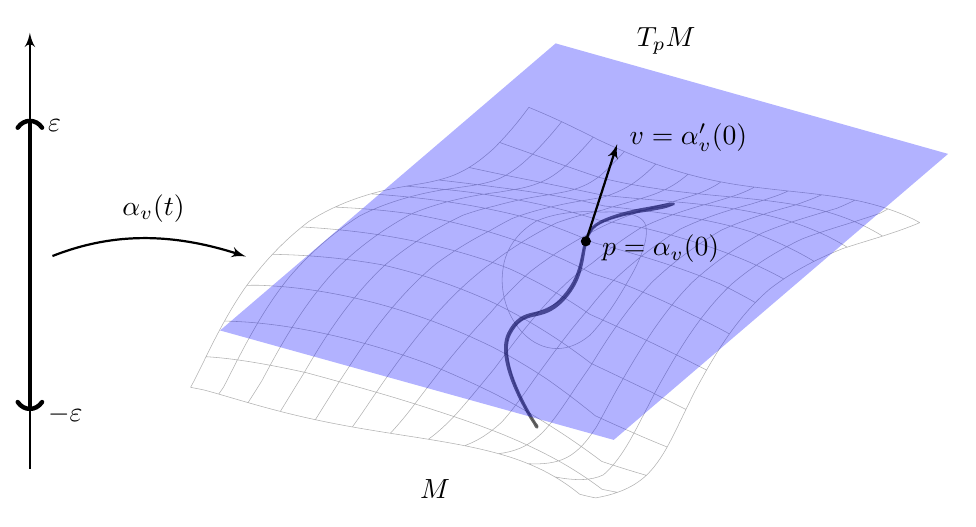
\begin{tikzpicture}[y=0.80pt, x=0.8pt,yscale=-1,scale=0.6, inner sep=0pt, outer sep=0pt]
\begin{scope}[shift={(-1.89918,-548.35592)}]% layer1
  \begin{scope}[shift={(-2166.7421,1235.8195)}]% g5925
    % path3481
    \path[draw=black,line join=miter,line cap=butt,line width=0.800pt,-latex']
      (2175.4461,-347.9786) -- (2175.4461,-676.1636);

    % path4477
    \path[fill=c666666] (2654.3031,-547.6441) .. controls (2647.4348,-546.2761) and
      (2640.5557,-545.0121) .. (2633.6677,-543.7951) .. controls
      (2626.6105,-542.2353) and (2619.5437,-540.4849) .. (2612.6819,-538.0226) ..
      controls (2609.7638,-536.9762) and (2606.8555,-535.7845) ..
      (2604.0836,-534.2680) .. controls (2604.0836,-534.2680) and
      (2604.0836,-534.2680) .. (2604.0836,-534.2680) .. controls
      (2601.9535,-533.1180) and (2599.8112,-531.7174) .. (2598.1005,-529.7703) ..
      controls (2597.8555,-529.4851) and (2597.6192,-529.1943) ..
      (2597.3914,-528.8983) .. controls (2595.1385,-525.9724) and
      (2593.6741,-522.5662) .. (2592.7057,-519.1105) .. controls
      (2592.7057,-519.1105) and (2592.7057,-519.1105) .. (2592.7057,-519.1105) ..
      controls (2591.5367,-514.9696) and (2590.8884,-510.7695) ..
      (2590.0477,-506.6825) .. controls (2590.0477,-506.6825) and
      (2590.0477,-506.6825) .. (2590.0477,-506.6825) .. controls
      (2589.0730,-501.9673) and (2587.8395,-497.3211) .. (2585.9734,-492.9636) ..
      controls (2583.6915,-487.6173) and (2580.4686,-482.6851) ..
      (2576.6167,-478.3090) .. controls (2575.6736,-477.2418) and
      (2574.6936,-476.2055) .. (2573.6743,-475.2150) .. controls
      (2570.9522,-472.5697) and (2567.8955,-470.3072) .. (2564.5128,-468.7394) ..
      controls (2561.2981,-467.2287) and (2557.7301,-466.4253) ..
      (2554.1022,-465.5946) .. controls (2554.1022,-465.5946) and
      (2554.1022,-465.5946) .. (2554.1022,-465.5946) .. controls
      (2550.7693,-464.8555) and (2547.3088,-463.8471) .. (2544.2156,-461.8055) ..
      controls (2540.0204,-458.9361) and (2537.0877,-454.7156) ..
      (2534.9228,-450.4212) .. controls (2534.9228,-450.4212) and
      (2534.9228,-450.4212) .. (2534.9228,-450.4212) .. controls
      (2533.2896,-447.1992) and (2532.5434,-443.6624) .. (2532.3848,-440.2058) ..
      controls (2532.3848,-440.2058) and (2532.3848,-440.2058) ..
      (2532.3848,-440.2058) .. controls (2532.3298,-439.0688) and
      (2532.3288,-437.9355) .. (2532.3748,-436.8088) .. controls
      (2532.4900,-434.0474) and (2532.8683,-431.3244) .. (2533.3993,-428.6666) ..
      controls (2533.3993,-428.6666) and (2533.3993,-428.6666) ..
      (2533.3993,-428.6666) .. controls (2535.0563,-420.3517) and
      (2538.0833,-412.4552) .. (2541.5661,-404.8920) .. controls
      (2541.5661,-404.8920) and (2541.5661,-404.8920) .. (2541.5661,-404.8920) ..
      controls (2544.6157,-398.2597) and (2548.0751,-391.8409) ..
      (2551.8220,-385.6202) .. controls (2551.8220,-385.6202) and
      (2551.8220,-385.6202) .. (2551.8220,-385.6202) .. controls
      (2552.7897,-384.0942) and (2553.7585,-382.5695) .. (2554.7286,-381.0460) ..
      controls (2556.5696,-375.7251) and (2560.6249,-378.5649) ..
      (2556.7431,-382.4256) .. controls (2555.8170,-383.9070) and
      (2554.8921,-385.3895) .. (2553.9684,-386.8732) .. controls
      (2553.9684,-386.8732) and (2553.9684,-386.8732) .. (2553.9684,-386.8732) ..
      controls (2550.3156,-393.0527) and (2546.9563,-399.4115) ..
      (2544.0122,-405.9611) .. controls (2544.0122,-405.9611) and
      (2544.0122,-405.9611) .. (2544.0122,-405.9611) .. controls
      (2540.6472,-413.4566) and (2537.7487,-421.1787) .. (2536.2304,-429.1892) ..
      controls (2536.2304,-429.1892) and (2536.2304,-429.1892) ..
      (2536.2304,-429.1892) .. controls (2535.7703,-431.6209) and
      (2535.4388,-434.0735) .. (2535.3302,-436.5215) .. controls
      (2535.2782,-437.6974) and (2535.2822,-438.8723) .. (2535.3522,-440.0422) ..
      controls (2535.3522,-440.0422) and (2535.3522,-440.0422) ..
      (2535.3522,-440.0422) .. controls (2535.5468,-443.2067) and
      (2536.2191,-446.3448) .. (2537.6584,-449.0533) .. controls
      (2537.6584,-449.0533) and (2537.6584,-449.0533) .. (2537.6584,-449.0533) ..
      controls (2539.8042,-453.0859) and (2542.4431,-456.9005) ..
      (2546.0402,-459.2081) .. controls (2548.5715,-460.8970) and
      (2551.6804,-461.7164) .. (2554.8889,-462.4430) .. controls
      (2554.8889,-462.4430) and (2554.8889,-462.4430) .. (2554.8889,-462.4430) ..
      controls (2558.5246,-463.2325) and (2562.3057,-464.0883) ..
      (2565.9500,-465.7505) .. controls (2569.4093,-467.3620) and
      (2572.5242,-469.5570) .. (2575.2820,-472.0923) .. controls
      (2576.6385,-473.3393) and (2577.9236,-474.6752) .. (2579.1353,-476.0703) ..
      controls (2583.1324,-480.6421) and (2586.4869,-485.9718) ..
      (2588.7968,-491.7770) .. controls (2590.6479,-496.4534) and
      (2591.7953,-501.3286) .. (2592.6508,-506.1573) .. controls
      (2592.6508,-506.1573) and (2592.6508,-506.1573) .. (2592.6508,-506.1573) ..
      controls (2593.4045,-510.3787) and (2593.9369,-514.5309) ..
      (2594.9806,-518.4549) .. controls (2595.8940,-521.8586) and
      (2597.2629,-525.1111) .. (2599.3563,-527.7167) .. controls
      (2599.5014,-527.8974) and (2599.6502,-528.0749) .. (2599.8026,-528.2490) ..
      controls (2601.2215,-529.9068) and (2603.1719,-531.1138) ..
      (2605.1900,-532.1913) .. controls (2607.8550,-533.5986) and
      (2610.6738,-534.6643) .. (2613.5273,-535.6002) .. controls
      (2620.3160,-537.8252) and (2627.2293,-539.2431) .. (2634.2532,-540.6061) ..
      controls (2640.3183,-541.5120) and (2646.4251,-542.5268) ..
      (2652.6920,-543.8088) .. controls (2655.6118,-544.4727) and
      (2661.0465,-546.3075) .. (2660.8879,-547.5775) .. controls
      (2660.8879,-547.5775) and (2660.8879,-547.5775) .. (2660.8879,-547.5775) ..
      controls (2660.8879,-547.5775) and (2660.8879,-547.5775) ..
      (2660.8879,-547.5775) .. controls (2660.8879,-547.5774) and
      (2660.8879,-547.5773) .. (2660.8880,-547.5773) .. controls
      (2660.8880,-547.5772) and (2660.8880,-547.5772) .. (2660.8880,-547.5771) ..
      controls (2660.8880,-547.5771) and (2660.8880,-547.5770) ..
      (2660.8880,-547.5770) .. controls (2660.8880,-547.5770) and
      (2660.8880,-547.5770) .. (2660.8880,-547.5769) .. controls
      (2660.8880,-547.5769) and (2660.8880,-547.5768) .. (2660.8880,-547.5767) ..
      controls (2660.8880,-547.5767) and (2660.8880,-547.5766) ..
      (2660.8881,-547.5766) .. controls (2660.8881,-547.5765) and
      (2660.8881,-547.5764) .. (2660.8881,-547.5764) .. controls
      (2660.8881,-547.5764) and (2660.8881,-547.5763) .. (2660.8881,-547.5763) ..
      controls (2660.8881,-547.5763) and (2660.8881,-547.5762) ..
      (2660.8881,-547.5762) .. controls (2660.8881,-547.5762) and
      (2660.8881,-547.5761) .. (2660.8881,-547.5760) .. controls
      (2660.8881,-547.5760) and (2660.8881,-547.5759) .. (2660.8881,-547.5759) ..
      controls (2660.8882,-547.5758) and (2660.8882,-547.5757) ..
      (2660.8882,-547.5757) .. controls (2660.8882,-547.5756) and
      (2660.8882,-547.5756) .. (2660.8882,-547.5756) .. controls
      (2660.8882,-547.5756) and (2660.8882,-547.5755) .. (2660.8882,-547.5755) ..
      controls (2660.8882,-547.5754) and (2660.8882,-547.5754) ..
      (2660.8882,-547.5753) .. controls (2660.8882,-547.5753) and
      (2660.8882,-547.5752) .. (2660.8882,-547.5751) .. controls
      (2660.8883,-547.5751) and (2660.8883,-547.5750) .. (2660.8883,-547.5750) ..
      controls (2661.0734,-546.2264) and (2661.0750,-546.2150) ..
      (2660.8883,-547.5880) .. controls (2660.8883,-547.5880) and
      (2660.8883,-547.5880) .. (2660.8883,-547.5880) .. controls
      (2660.8503,-547.8383) and (2660.5935,-548.0662) .. (2660.0525,-548.2582) ..
      controls (2658.3184,-548.4115) and (2656.1906,-547.9767) ..
      (2654.3031,-547.6441) -- cycle;

    % path4477-5
    \path[draw=black,opacity=0.300,line join=miter,line cap=butt,line width=0.200pt]
      (2557.4416,-379.4465) .. controls (2557.4416,-379.4465) and
      (2555.9117,-381.5302) .. (2553.5831,-385.2230) .. controls
      (2553.1305,-385.9406) and (2552.6477,-386.7201) .. (2552.1406,-387.5593) ..
      controls (2549.8734,-391.3494) and (2547.1202,-396.2918) ..
      (2544.4938,-401.9720) .. controls (2541.8674,-407.6522) and
      (2539.3776,-414.0709) .. (2537.6726,-420.6592) .. controls
      (2537.5826,-420.9440) and (2537.4950,-421.2289) .. (2537.4087,-421.5139) ..
      controls (2537.4087,-421.5139) and (2537.4087,-421.5139) ..
      (2537.4086,-421.5139) .. controls (2535.1383,-429.2807) and
      (2533.9052,-437.0626) .. (2534.8097,-443.6623) .. controls
      (2535.9345,-451.8698) and (2540.6337,-456.8091) .. (2546.6297,-460.5100) ..
      controls (2552.5389,-464.1449) and (2559.6892,-466.5689) ..
      (2566.2336,-469.7023) .. controls (2569.5058,-471.2690) and
      (2572.6335,-473.0146) .. (2575.4307,-475.1584) .. controls
      (2578.2278,-477.3022) and (2580.6946,-479.8476) .. (2582.6743,-482.9538) ..
      controls (2584.3182,-485.5332) and (2585.6665,-488.2920) ..
      (2586.8253,-491.1236) .. controls (2588.1860,-494.4074) and
      (2589.1383,-497.8791) .. (2589.9295,-501.3506) .. controls
      (2590.7206,-504.8222) and (2591.3501,-508.2929) .. (2592.0547,-511.6149) ..
      controls (2593.4638,-518.2589) and (2595.1788,-524.2773) ..
      (2599.0196,-528.9495) .. controls (2600.1853,-530.0014) and
      (2601.5172,-530.9322) .. (2603.0578,-531.7408) .. controls
      (2603.0708,-531.7488) and (2603.0838,-531.7571) .. (2603.0968,-531.7653) ..
      controls (2607.8315,-534.7591) and (2615.6227,-537.3792) ..
      (2623.9788,-539.5326) .. controls (2632.3349,-541.6860) and
      (2641.2552,-543.3918) .. (2648.2547,-544.6083) .. controls
      (2655.7818,-545.8840) and (2661.0289,-546.5606) ..
      (2661.0289,-546.5606)(2609.5231,-463.6069) .. controls (2605.4389,-457.9478)
      and (2601.2840,-452.8429) .. (2597.0665,-448.4899) .. controls
      (2592.8950,-445.0147) and (2588.6416,-442.4203) .. (2584.3419,-440.7433) ..
      controls (2580.0423,-439.0663) and (2575.6971,-438.3020) ..
      (2571.3942,-438.4250) .. controls (2562.7884,-438.6711) and
      (2554.3157,-442.4544) .. (2547.1738,-449.5339) .. controls
      (2547.1738,-449.5339) and (2547.1738,-449.5339) .. (2547.1738,-449.5339) ..
      controls (2544.2621,-452.4174) and (2541.5784,-455.8513) ..
      (2539.2379,-459.7983) .. controls (2535.7617,-465.6605) and
      (2533.3254,-472.1897) .. (2532.0406,-478.8915) .. controls
      (2530.7558,-485.5933) and (2530.6273,-492.4581) .. (2531.6999,-498.9753) ..
      controls (2532.3997,-504.5215) and (2534.1740,-509.9253) ..
      (2536.9822,-514.9174) .. controls (2539.7904,-519.9094) and
      (2543.6323,-524.4880) .. (2548.3806,-528.4896) .. controls
      (2548.3806,-528.4896) and (2548.3806,-528.4896) .. (2548.3806,-528.4896) ..
      controls (2550.9433,-530.6429) and (2553.7685,-532.6294) ..
      (2556.8281,-534.4361) .. controls (2558.1212,-535.0011) and
      (2559.4506,-535.5304) .. (2560.8146,-536.0252) .. controls
      (2568.4231,-538.7854) and (2576.3498,-540.2425) .. (2584.0598,-540.9704) ..
      controls (2591.7697,-541.6984) and (2599.2680,-541.6840) ..
      (2606.0968,-541.1086) .. controls (2612.5489,-541.4262) and
      (2618.4768,-541.2352) .. (2623.4991,-540.4719) .. controls
      (2628.5214,-539.7087) and (2632.6344,-538.3852) .. (2635.4554,-536.1979) ..
      controls (2637.9757,-534.2438) and (2639.2589,-531.7361) ..
      (2639.4503,-528.5414) .. controls (2639.8948,-523.5478) and
      (2638.7278,-517.6081) .. (2636.3206,-510.9120) .. controls
      (2633.9134,-504.2160) and (2630.2778,-496.7536) .. (2625.6297,-489.0176) ..
      controls (2620.9342,-480.7753) and (2615.5749,-471.9931) ..
      (2609.5227,-463.6069) -- cycle(2551.0375,-619.9898) .. controls
      (2560.1488,-616.2889) and (2569.0646,-612.3322) .. (2577.8055,-608.2124) ..
      controls (2586.5463,-604.0927) and (2595.1130,-599.8111) ..
      (2603.5722,-595.5063) .. controls (2620.2718,-587.7073) and
      (2636.7772,-580.4591) .. (2654.0437,-574.7624) .. controls
      (2663.7404,-571.5502) and (2673.5406,-568.7649) .. (2683.4727,-566.4565) ..
      controls (2693.4047,-564.1480) and (2703.4695,-562.3199) ..
      (2713.6568,-560.9102) .. controls (2713.6568,-560.9102) and
      (2713.6568,-560.9102) .. (2713.6568,-560.9102) .. controls
      (2725.3388,-559.3015) and (2737.0570,-558.0434) .. (2748.7310,-556.7874) ..
      controls (2760.4050,-555.5313) and (2772.0313,-554.2785) ..
      (2783.5678,-552.5011) .. controls (2783.5678,-552.5011) and
      (2783.5678,-552.5011) .. (2783.5678,-552.5011) .. controls
      (2802.3924,-549.5161) and (2821.1223,-544.9625) .. (2839.7604,-536.1878) ..
      controls (2841.6324,-535.2444) and (2843.4951,-534.2511) ..
      (2845.3489,-533.2044)(2529.0460,-593.5632) .. controls (2535.8939,-591.1711)
      and (2542.7283,-588.7463) .. (2549.5614,-586.3207) .. controls
      (2557.0223,-583.6253) and (2564.4828,-580.9325) .. (2571.9733,-578.3000) ..
      controls (2582.7318,-574.5060) and (2593.4142,-570.7743) ..
      (2604.0347,-567.2631) .. controls (2613.1901,-564.9797) and
      (2622.3890,-562.9937) .. (2631.6612,-561.3621) .. controls
      (2631.6612,-561.3621) and (2631.6612,-561.3621) .. (2631.6612,-561.3621) ..
      controls (2643.2120,-559.3352) and (2654.7600,-557.6774) ..
      (2666.2705,-556.3037) .. controls (2677.7810,-554.9299) and
      (2689.2522,-553.8417) .. (2700.6421,-552.8333) .. controls
      (2700.6421,-552.8333) and (2700.6421,-552.8333) .. (2700.6421,-552.8333) ..
      controls (2719.2116,-551.0789) and (2737.7414,-549.2934) ..
      (2756.1688,-545.9060) .. controls (2765.1932,-544.1498) and
      (2774.0481,-541.9570) .. (2782.7358,-539.0789) .. controls
      (2794.5116,-535.1588) and (2806.0518,-530.0571) ..
      (2817.3420,-523.0760)(2506.0329,-574.7403) .. controls (2512.2713,-573.3960)
      and (2518.5608,-572.0460) .. (2524.8907,-570.6950) .. controls
      (2524.8907,-570.6950) and (2524.8907,-570.6950) .. (2524.8907,-570.6950) ..
      controls (2532.6925,-569.0624) and (2540.4765,-567.4691) ..
      (2548.2338,-565.9403) .. controls (2549.3394,-565.7228) and
      (2550.4435,-565.5052) .. (2551.5460,-565.2873) .. controls
      (2570.6633,-561.4203) and (2589.3152,-557.5136) .. (2607.2708,-553.7521) ..
      controls (2607.2708,-553.7521) and (2607.2708,-553.7521) ..
      (2607.2708,-553.7521) .. controls (2610.9659,-553.3746) and
      (2614.6498,-553.0211) .. (2618.3216,-552.6898) .. controls
      (2618.3216,-552.6898) and (2618.3216,-552.6898) .. (2618.3217,-552.6898) ..
      controls (2636.9346,-550.9028) and (2655.4128,-549.4679) ..
      (2673.7306,-547.7093) .. controls (2682.9510,-546.7354) and
      (2692.0307,-545.6532) .. (2700.9524,-544.3165) .. controls
      (2700.9524,-544.3165) and (2700.9524,-544.3165) .. (2700.9524,-544.3165) ..
      controls (2716.5658,-541.9373) and (2731.8693,-538.9413) ..
      (2746.8230,-534.3626) .. controls (2761.7766,-529.7839) and
      (2776.3758,-523.6079) .. (2790.6383,-514.7359)(2483.1162,-565.3088) ..
      controls (2497.8946,-563.6393) and (2512.7707,-561.8330) ..
      (2527.5453,-559.8151) .. controls (2527.5453,-559.8151) and
      (2527.5453,-559.8151) .. (2527.5453,-559.8151) .. controls
      (2529.5186,-559.5711) and (2531.4853,-559.3253) .. (2533.4450,-559.0775) ..
      controls (2540.3646,-558.1642) and (2547.2171,-557.1945) ..
      (2553.9903,-556.1634) .. controls (2566.6592,-554.1874) and
      (2579.0520,-552.0016) .. (2591.1217,-549.5906) .. controls
      (2596.7885,-548.3724) and (2602.3588,-547.0945) .. (2607.8283,-545.7556) ..
      controls (2607.8283,-545.7556) and (2607.8283,-545.7556) ..
      (2607.8283,-545.7556) .. controls (2611.5735,-545.3482) and
      (2615.2950,-544.9325) .. (2618.9918,-544.5041) .. controls
      (2618.9918,-544.5041) and (2618.9918,-544.5041) .. (2618.9918,-544.5041) ..
      controls (2636.4873,-542.4319) and (2653.6416,-540.2759) ..
      (2670.4282,-537.4234) .. controls (2687.2147,-534.5708) and
      (2703.6297,-531.0133) .. (2719.6656,-525.8463) .. controls
      (2719.6656,-525.8463) and (2719.6656,-525.8463) .. (2719.6656,-525.8463) ..
      controls (2735.3794,-520.0962) and (2750.7650,-513.1042) ..
      (2765.7888,-504.0713)(2458.6046,-560.6457) .. controls (2472.5564,-559.6603)
      and (2486.5880,-558.4446) .. (2500.5584,-556.8559) .. controls
      (2509.6141,-555.7300) and (2518.6207,-554.4285) .. (2527.5350,-552.9276) ..
      controls (2529.7261,-552.5827) and (2531.9052,-552.2263) ..
      (2534.0718,-551.8581) .. controls (2534.0718,-551.8581) and
      (2534.0718,-551.8581) .. (2534.0718,-551.8581) .. controls
      (2540.3866,-550.7705) and (2546.6176,-549.6013) .. (2552.7574,-548.3467) ..
      controls (2570.6581,-544.6339) and (2587.7773,-540.1972) ..
      (2604.0464,-535.0449) .. controls (2604.0464,-535.0449) and
      (2604.0464,-535.0449) .. (2604.0464,-535.0449) .. controls
      (2616.3359,-533.0928) and (2628.4299,-530.9767) .. (2640.3322,-528.5397) ..
      controls (2640.3322,-528.5397) and (2640.3322,-528.5397) ..
      (2640.3322,-528.5397) .. controls (2658.1483,-524.0538) and
      (2675.6056,-519.0908) .. (2692.7077,-513.0371) .. controls
      (2709.8098,-506.9834) and (2726.5550,-499.8292) ..
      (2742.9340,-490.8132)(2432.1021,-554.8541) .. controls (2432.4550,-554.8313)
      and (2432.8080,-554.8084) .. (2433.1611,-554.7852) .. controls
      (2433.1611,-554.7852) and (2433.1611,-554.7852) .. (2433.1611,-554.7852) ..
      controls (2435.3765,-554.6351) and (2437.5959,-554.4784) ..
      (2439.8192,-554.3143) .. controls (2453.9961,-553.2393) and
      (2468.2145,-551.8314) .. (2482.3621,-549.9352) .. controls
      (2496.5098,-548.0390) and (2510.5860,-545.6562) .. (2524.4602,-542.7147) ..
      controls (2524.4602,-542.7147) and (2524.4602,-542.7147) ..
      (2524.4602,-542.7147) .. controls (2532.9868,-540.9590) and
      (2541.3439,-538.9923) .. (2549.5165,-536.8108) .. controls
      (2552.5904,-535.9827) and (2555.6385,-535.1245) .. (2558.6603,-534.2363) ..
      controls (2558.6603,-534.2363) and (2558.6603,-534.2363) ..
      (2558.6603,-534.2363) .. controls (2573.2100,-529.3368) and
      (2587.1898,-523.8712) .. (2600.5985,-517.9157) .. controls
      (2600.5985,-517.9157) and (2600.5985,-517.9157) .. (2600.5985,-517.9157) ..
      controls (2616.7809,-513.6408) and (2632.6634,-509.1315) ..
      (2648.2792,-504.1437) .. controls (2663.8949,-499.1559) and
      (2679.2433,-493.6861) .. (2694.3431,-487.3820) .. controls
      (2703.4630,-482.9791) and (2712.5319,-478.2096) ..
      (2721.5663,-473.0566)(2405.1275,-544.9048) .. controls (2415.7449,-544.4183)
      and (2426.4408,-543.7302) .. (2437.2074,-542.7516) .. controls
      (2445.9059,-541.9438) and (2454.6053,-540.9386) .. (2463.2828,-539.7067) ..
      controls (2483.1049,-536.1782) and (2502.8661,-531.6027) ..
      (2522.2439,-525.8929) .. controls (2522.2439,-525.8929) and
      (2522.2439,-525.8929) .. (2522.2439,-525.8929) .. controls
      (2530.8300,-523.3317) and (2539.2472,-520.5465) .. (2547.4834,-517.5445) ..
      controls (2565.3552,-510.9953) and (2582.3717,-503.4221) ..
      (2598.5204,-495.0132) .. controls (2598.5204,-495.0132) and
      (2598.5204,-495.0132) .. (2598.5204,-495.0132) .. controls
      (2604.7771,-493.0528) and (2610.9915,-491.0547) .. (2617.1669,-489.0112) ..
      controls (2631.5269,-483.3512) and (2645.7445,-477.2695) ..
      (2659.8770,-470.6908) .. controls (2674.0094,-464.1122) and
      (2688.0564,-457.0256) .. (2702.0780,-449.4648)(2380.1526,-529.9402) ..
      controls (2398.5975,-528.9450) and (2417.3256,-527.1707) ..
      (2436.3532,-524.3666) .. controls (2450.6233,-522.2363) and
      (2464.9367,-519.5033) .. (2479.1818,-516.1145) .. controls
      (2493.4269,-512.7257) and (2507.6027,-508.6810) .. (2521.5736,-503.9700) ..
      controls (2521.5736,-503.9700) and (2521.5736,-503.9700) ..
      (2521.5736,-503.9700) .. controls (2526.5921,-502.2345) and
      (2531.5523,-500.4097) .. (2536.4512,-498.4978) .. controls
      (2539.8725,-496.9625) and (2543.2664,-495.3754) .. (2546.6322,-493.7378) ..
      controls (2564.1946,-485.1649) and (2580.9871,-475.2109) ..
      (2597.0033,-464.1823) .. controls (2597.0033,-464.1823) and
      (2597.0033,-464.1823) .. (2597.0033,-464.1822) .. controls
      (2611.7785,-457.7035) and (2626.4427,-450.9557) .. (2641.0624,-443.9492) ..
      controls (2655.6821,-436.9427) and (2670.2568,-429.6668) ..
      (2684.8553,-422.2144)(2358.0762,-509.3621) .. controls (2370.9169,-509.1442)
      and (2383.9063,-508.4796) .. (2397.0891,-507.2887) .. controls
      (2410.2718,-506.0979) and (2423.6476,-504.3808) .. (2437.2012,-502.0610) ..
      controls (2438.1274,-501.9007) and (2439.0539,-501.7375) ..
      (2439.9806,-501.5714) .. controls (2439.9807,-501.5714) and
      (2439.9807,-501.5714) .. (2439.9807,-501.5714) .. controls
      (2467.0451,-495.5066) and (2494.5140,-486.3828) .. (2521.4148,-474.3073) ..
      controls (2521.4148,-474.3073) and (2521.4148,-474.3073) ..
      (2521.4148,-474.3073) .. controls (2529.9613,-470.2845) and
      (2538.3611,-465.9447) .. (2546.5992,-461.3111) .. controls
      (2564.4750,-451.2333) and (2581.5855,-439.7644) .. (2597.8980,-427.2529) ..
      controls (2597.8980,-427.2529) and (2597.8981,-427.2529) ..
      (2597.8981,-427.2529) .. controls (2612.1670,-420.5422) and
      (2626.3870,-413.7629) .. (2640.6203,-406.9538) .. controls
      (2640.6203,-406.9538) and (2640.6203,-406.9538) .. (2640.6203,-406.9538) ..
      controls (2641.2366,-406.6554) and (2641.8532,-406.3571) ..
      (2642.4701,-406.0589) .. controls (2651.3405,-401.5252) and
      (2660.2957,-397.0279) .. (2669.3361,-392.5912)(2338.8050,-486.0168) ..
      controls (2341.5245,-486.0654) and (2344.2510,-486.0913) ..
      (2346.9860,-486.0944) .. controls (2346.9860,-486.0944) and
      (2346.9860,-486.0944) .. (2346.9860,-486.0944) .. controls
      (2350.5373,-485.9835) and (2354.1014,-485.8178) .. (2357.6824,-485.5982) ..
      controls (2370.6165,-484.8071) and (2383.7711,-483.2706) ..
      (2397.2306,-480.9871) .. controls (2410.6901,-478.7035) and
      (2424.4533,-475.6743) .. (2438.4969,-471.8869) .. controls
      (2438.4969,-471.8869) and (2438.4970,-471.8869) .. (2438.4970,-471.8869) ..
      controls (2466.6391,-464.2451) and (2495.4391,-453.4434) ..
      (2523.5085,-439.6779) .. controls (2523.5085,-439.6779) and
      (2523.5085,-439.6779) .. (2523.5085,-439.6779) .. controls
      (2532.1635,-435.2094) and (2540.6703,-430.4408) .. (2549.0096,-425.3918) ..
      controls (2553.7157,-422.5376) and (2558.3691,-419.5944) ..
      (2562.9675,-416.5666) .. controls (2562.9675,-416.5666) and
      (2562.9675,-416.5666) .. (2562.9675,-416.5666) .. controls
      (2563.6008,-416.1470) and (2564.2334,-415.7258) .. (2564.8652,-415.3032) ..
      controls (2577.1820,-406.6474) and (2589.2558,-397.4700) ..
      (2601.0254,-387.8699) .. controls (2612.5986,-382.5252) and
      (2624.2630,-377.3258) .. (2636.0199,-372.2662) .. controls
      (2642.3935,-369.5291) and (2648.7871,-366.8725) ..
      (2655.2016,-364.2920)(2321.9281,-459.0707) .. controls (2334.8340,-458.8823)
      and (2347.9349,-457.7952) .. (2361.4439,-455.9928) .. controls
      (2374.1631,-454.2992) and (2387.2334,-451.9251) .. (2400.6787,-448.9247) ..
      controls (2414.1239,-445.9242) and (2427.9428,-442.2984) ..
      (2442.0508,-438.0467) .. controls (2442.0508,-438.0467) and
      (2442.0508,-438.0467) .. (2442.0508,-438.0467) .. controls
      (2452.4643,-434.8895) and (2462.9654,-431.3767) .. (2473.4737,-427.5124) ..
      controls (2473.4737,-427.5124) and (2473.4737,-427.5124) ..
      (2473.4737,-427.5124) .. controls (2474.2349,-427.2284) and
      (2474.9964,-426.9426) .. (2475.7582,-426.6552) .. controls
      (2492.7422,-419.7284) and (2510.0339,-411.9978) .. (2527.0870,-403.4535) ..
      controls (2535.8479,-398.8456) and (2544.5011,-394.0134) ..
      (2553.0026,-388.9547) .. controls (2554.4300,-388.1042) and
      (2555.8532,-387.2474) .. (2557.2720,-386.3841) .. controls
      (2557.2720,-386.3841) and (2557.2720,-386.3841) .. (2557.2720,-386.3841) ..
      controls (2574.2363,-376.0864) and (2590.5040,-365.1423) ..
      (2605.9389,-353.4476) .. controls (2612.3877,-351.2980) and
      (2618.8359,-349.2283) .. (2625.2869,-347.2224) .. controls
      (2630.0364,-345.7695) and (2634.7709,-344.3565) ..
      (2639.4948,-342.9764)(2308.0680,-432.2921) .. controls (2317.4344,-431.7290)
      and (2326.9458,-430.6363) .. (2336.7039,-429.1758) .. controls
      (2346.4620,-427.7154) and (2356.4665,-425.8883) .. (2366.7674,-423.8093) ..
      controls (2371.7186,-422.8120) and (2376.7358,-421.7481) ..
      (2381.8180,-420.6236) .. controls (2381.8180,-420.6236) and
      (2381.8180,-420.6236) .. (2381.8180,-420.6236) .. controls
      (2382.5089,-420.4666) and (2383.2014,-420.3085) .. (2383.8953,-420.1493) ..
      controls (2393.5504,-417.5640) and (2403.6448,-414.7805) ..
      (2414.0971,-411.8404) .. controls (2424.5494,-408.9002) and
      (2435.3584,-405.8030) .. (2446.3927,-402.5331) .. controls
      (2446.3927,-402.5331) and (2446.3927,-402.5331) .. (2446.3928,-402.5331) ..
      controls (2452.9812,-400.5695) and (2459.6236,-398.5387) ..
      (2466.2837,-396.4362) .. controls (2466.2837,-396.4362) and
      (2466.2837,-396.4362) .. (2466.2837,-396.4362) .. controls
      (2488.4527,-389.4491) and (2510.7414,-382.0569) .. (2531.8186,-373.6242) ..
      controls (2531.8186,-373.6242) and (2531.8186,-373.6242) ..
      (2531.8186,-373.6242) .. controls (2536.4007,-371.7364) and
      (2540.9214,-369.7956) .. (2545.3746,-367.7922) .. controls
      (2549.3584,-366.0220) and (2553.2764,-364.2054) .. (2557.1280,-362.3350) ..
      controls (2574.8591,-353.7135) and (2591.1579,-343.9200) ..
      (2606.1952,-332.4437) .. controls (2610.0595,-331.6752) and
      (2613.9157,-330.9185) .. (2617.7682,-330.1663)(2589.3299,-328.7502) ..
      controls (2593.5543,-327.6320) and (2597.5655,-326.7028) ..
      (2601.3584,-325.9980) .. controls (2610.4938,-327.6063) and
      (2618.5129,-329.9693) .. (2625.4639,-333.3694) .. controls
      (2632.4148,-336.7695) and (2638.2968,-341.2080) .. (2643.2475,-346.8678) ..
      controls (2649.2485,-353.7202) and (2654.3668,-362.1923) ..
      (2659.3356,-372.1263) .. controls (2659.3356,-372.1263) and
      (2659.3356,-372.1263) .. (2659.3356,-372.1263) .. controls
      (2664.6782,-382.6525) and (2669.9842,-394.1952) .. (2675.9221,-405.9773) ..
      controls (2675.9221,-405.9773) and (2675.9221,-405.9773) ..
      (2675.9221,-405.9773) .. controls (2676.0731,-406.2744) and
      (2676.2246,-406.5715) .. (2676.3765,-406.8686) .. controls
      (2680.3336,-414.2261) and (2684.3833,-421.5486) .. (2688.6079,-428.6506) ..
      controls (2692.8326,-435.7526) and (2697.2324,-442.6337) ..
      (2701.8574,-449.1533) .. controls (2706.4824,-455.6728) and
      (2711.3326,-461.8306) .. (2716.4250,-467.5349) .. controls
      (2721.5174,-473.2393) and (2726.8518,-478.4902) .. (2732.4119,-483.2480) ..
      controls (2740.6159,-489.5663) and (2749.2549,-495.1770) ..
      (2758.3552,-500.1721) .. controls (2767.4554,-505.1673) and
      (2777.0166,-509.5477) .. (2787.0087,-513.5371) .. controls
      (2787.0087,-513.5371) and (2787.0087,-513.5371) .. (2787.0087,-513.5371) ..
      controls (2794.6347,-516.0934) and (2802.4476,-518.4465) ..
      (2810.4378,-520.9161) .. controls (2818.4280,-523.3858) and
      (2826.5957,-525.9731) .. (2834.9214,-529.0679) .. controls
      (2834.9214,-529.0679) and (2834.9214,-529.0679) .. (2834.9214,-529.0679) ..
      controls (2838.3738,-530.3474) and (2841.8463,-531.7124) ..
      (2845.3494,-533.2042)(2570.7184,-341.7897) .. controls (2578.2857,-340.3539)
      and (2585.1143,-339.6146) .. (2591.1838,-339.8051) .. controls
      (2597.2533,-339.9955) and (2602.5636,-341.1164) .. (2607.1547,-343.3398) ..
      controls (2608.6519,-344.6235) and (2610.0863,-345.9827) ..
      (2611.4601,-347.4204) .. controls (2617.9026,-354.1623) and
      (2623.4647,-362.4798) .. (2628.8237,-372.3006) .. controls
      (2628.8237,-372.3006) and (2628.8237,-372.3006) .. (2628.8237,-372.3006) ..
      controls (2634.5786,-382.7069) and (2640.2337,-394.1936) ..
      (2646.4480,-406.0620) .. controls (2646.4480,-406.0620) and
      (2646.4480,-406.0620) .. (2646.4480,-406.0620) .. controls
      (2646.6053,-406.3611) and (2646.7630,-406.6603) .. (2646.9211,-406.9597) ..
      controls (2655.1486,-421.7843) and (2663.6528,-436.6535) ..
      (2672.9761,-450.2706) .. controls (2677.6377,-457.0791) and
      (2682.4970,-463.5837) .. (2687.5778,-469.6829) .. controls
      (2692.6587,-475.7821) and (2697.9611,-481.4756) .. (2703.4795,-486.7070) ..
      controls (2703.4795,-486.7070) and (2703.4795,-486.7070) ..
      (2703.4795,-486.7070) .. controls (2711.5722,-493.6352) and
      (2720.0363,-499.9070) .. (2728.9002,-505.5699) .. controls
      (2737.7641,-511.2327) and (2747.0276,-516.2873) .. (2756.6663,-520.8972) ..
      controls (2756.6663,-520.8972) and (2756.6663,-520.8972) ..
      (2756.6663,-520.8972) .. controls (2764.0640,-523.7385) and
      (2771.6151,-526.2547) .. (2779.3091,-528.6900) .. controls
      (2787.0031,-531.1254) and (2794.8400,-533.4810) .. (2802.8003,-536.0611) ..
      controls (2802.8003,-536.0611) and (2802.8003,-536.0611) ..
      (2802.8003,-536.0611) .. controls (2807.0064,-537.4080) and
      (2811.2146,-538.7947) .. (2815.4402,-540.2874) .. controls
      (2815.4402,-540.2874) and (2815.4402,-540.2874) .. (2815.4402,-540.2874) ..
      controls (2817.4227,-541.3160) and (2819.4033,-542.3992) ..
      (2821.3868,-543.5522)(2550.4477,-351.7879) .. controls (2552.0441,-351.6948)
      and (2553.6053,-351.6371) .. (2555.1310,-351.6177) .. controls
      (2565.6686,-351.4798) and (2574.4831,-353.1906) .. (2581.6142,-357.5104) ..
      controls (2587.7663,-361.2745) and (2593.1234,-366.8051) ..
      (2598.2692,-374.1115) .. controls (2598.2692,-374.1115) and
      (2598.2692,-374.1115) .. (2598.2692,-374.1115) .. controls
      (2599.5303,-375.8775) and (2600.7849,-377.7161) .. (2602.0411,-379.6201) ..
      controls (2606.7344,-387.9532) and (2611.4440,-396.8417) ..
      (2616.4483,-405.9983) .. controls (2616.4483,-405.9983) and
      (2616.4483,-405.9983) .. (2616.4483,-405.9983) .. controls
      (2616.6116,-406.2971) and (2616.7752,-406.5961) .. (2616.9392,-406.8953) ..
      controls (2625.4627,-421.7125) and (2634.1697,-436.6962) ..
      (2643.5952,-450.6005) .. controls (2653.0207,-464.5048) and
      (2663.1658,-477.3205) .. (2674.1477,-488.3648) .. controls
      (2674.1478,-488.3648) and (2674.1478,-488.3648) .. (2674.1478,-488.3648) ..
      controls (2682.1745,-495.6811) and (2690.5169,-502.3896) ..
      (2699.2031,-508.5079) .. controls (2707.8894,-514.6262) and
      (2716.9192,-520.1549) .. (2726.2709,-525.2154) .. controls
      (2726.2709,-525.2154) and (2726.2709,-525.2154) .. (2726.2709,-525.2154) ..
      controls (2733.4750,-528.2875) and (2740.8019,-530.9624) ..
      (2748.2405,-533.4306) .. controls (2755.6792,-535.8988) and
      (2763.2294,-538.1612) .. (2770.8714,-540.4602) .. controls
      (2770.8714,-540.4602) and (2770.8714,-540.4602) .. (2770.8714,-540.4602) ..
      controls (2774.9136,-541.6527) and (2778.9359,-542.8203) ..
      (2782.9495,-544.0150) .. controls (2782.9495,-544.0150) and
      (2782.9495,-544.0150) .. (2782.9495,-544.0150) .. controls
      (2787.5148,-545.8793) and (2792.0306,-547.8740) ..
      (2796.5491,-550.1563)(2528.1858,-359.3075) .. controls (2529.5939,-359.4740)
      and (2530.9835,-359.6673) .. (2532.3533,-359.8893) .. controls
      (2539.2236,-361.1615) and (2545.3226,-363.3151) .. (2550.6465,-366.6198) ..
      controls (2552.4892,-367.7741) and (2554.2749,-369.0519) ..
      (2556.0150,-370.4569) .. controls (2560.4055,-373.9950) and
      (2564.5061,-378.3442) .. (2568.5012,-383.5227) .. controls
      (2568.5012,-383.5227) and (2568.5012,-383.5227) .. (2568.5012,-383.5227) ..
      controls (2574.4884,-391.1837) and (2580.3667,-400.0821) ..
      (2586.6959,-409.6870) .. controls (2586.6959,-409.6870) and
      (2586.6959,-409.6870) .. (2586.6959,-409.6870) .. controls
      (2586.8537,-409.9261) and (2587.0119,-410.1656) .. (2587.1704,-410.4054) ..
      controls (2590.7386,-415.5220) and (2594.3217,-420.7611) ..
      (2597.9681,-426.0179) .. controls (2605.0075,-437.5598) and
      (2612.2798,-448.8911) .. (2619.9749,-459.5142) .. controls
      (2627.6700,-470.1373) and (2635.7881,-480.0497) .. (2644.3757,-488.9476) ..
      controls (2644.3757,-488.9476) and (2644.3757,-488.9476) ..
      (2644.3757,-488.9476) .. controls (2652.3756,-496.4794) and
      (2660.6445,-503.4454) .. (2669.2083,-509.8449) .. controls
      (2677.7721,-516.2445) and (2686.6303,-522.0781) .. (2695.7611,-527.4397) ..
      controls (2695.7611,-527.4397) and (2695.7611,-527.4397) ..
      (2695.7611,-527.4397) .. controls (2702.8106,-530.6807) and
      (2709.9556,-533.4882) .. (2717.1839,-536.0165) .. controls
      (2724.4122,-538.5449) and (2731.7238,-540.7951) .. (2739.0982,-542.9678) ..
      controls (2739.0982,-542.9678) and (2739.0982,-542.9678) ..
      (2739.0982,-542.9678) .. controls (2743.0014,-544.0903) and
      (2746.8693,-545.1490) .. (2750.7100,-546.1863) .. controls
      (2750.7100,-546.1863) and (2750.7100,-546.1863) .. (2750.7100,-546.1863) ..
      controls (2756.5619,-548.2036) and (2762.2898,-550.2619) ..
      (2767.9888,-552.6443) .. controls (2769.1849,-553.1301) and
      (2770.3731,-553.6409) .. (2771.5553,-554.1781)(2502.7205,-365.2771) ..
      controls (2507.7643,-367.1862) and (2512.5550,-369.5251) ..
      (2517.0435,-372.4113) .. controls (2521.5617,-375.3394) and
      (2525.9480,-378.7565) .. (2530.2731,-382.7044) .. controls
      (2532.5587,-385.1158) and (2534.7990,-387.7226) .. (2537.0162,-390.5282) ..
      controls (2537.0162,-390.5282) and (2537.0162,-390.5282) ..
      (2537.0162,-390.5283) .. controls (2541.4912,-396.1221) and
      (2545.9305,-402.2226) .. (2550.5092,-408.6822) .. controls
      (2552.4717,-411.4461) and (2554.4597,-414.2753) .. (2556.4854,-417.1574) ..
      controls (2556.4854,-417.1574) and (2556.4854,-417.1574) ..
      (2556.4854,-417.1574) .. controls (2556.6527,-417.3963) and
      (2556.8202,-417.6354) .. (2556.9881,-417.8748) .. controls
      (2563.3740,-426.5192) and (2569.7894,-435.4106) .. (2576.4257,-444.1157) ..
      controls (2583.0619,-452.8207) and (2589.9202,-461.3360) ..
      (2597.1081,-469.3173) .. controls (2602.5831,-476.2715) and
      (2608.2501,-482.8626) .. (2614.1184,-489.0053) .. controls
      (2614.1184,-489.0053) and (2614.1184,-489.0053) .. (2614.1184,-489.0053) ..
      controls (2622.1223,-496.6274) and (2630.3598,-503.7163) ..
      (2638.8515,-510.2619) .. controls (2647.3432,-516.8074) and
      (2656.0887,-522.8100) .. (2665.0627,-528.3473) .. controls
      (2665.0627,-528.3473) and (2665.0627,-528.3473) .. (2665.0627,-528.3473) ..
      controls (2671.9995,-531.6949) and (2679.0078,-534.5955) ..
      (2686.0739,-537.1825) .. controls (2693.1400,-539.7694) and
      (2700.2639,-542.0436) .. (2707.4240,-544.1812) .. controls
      (2707.4240,-544.1812) and (2707.4240,-544.1812) .. (2707.4240,-544.1812) ..
      controls (2711.2154,-545.2834) and (2714.9602,-546.3017) ..
      (2718.6652,-547.2730) .. controls (2718.6653,-547.2730) and
      (2718.6653,-547.2730) .. (2718.6653,-547.2730) .. controls
      (2724.4702,-549.0920) and (2730.1276,-550.8540) .. (2735.7204,-552.8055) ..
      controls (2739.3388,-554.0155) and (2742.8566,-555.4176) ..
      (2746.3217,-557.0465)(2475.3873,-370.1476) .. controls (2477.3441,-371.5248)
      and (2479.2609,-372.9836) .. (2481.1336,-374.5329) .. controls
      (2488.0420,-380.2695) and (2494.7958,-387.0753) .. (2501.6256,-395.1051) ..
      controls (2501.6256,-395.1051) and (2501.6256,-395.1051) ..
      (2501.6257,-395.1051) .. controls (2508.9413,-403.6120) and
      (2516.4651,-412.8902) .. (2524.5293,-422.5683) .. controls
      (2524.5293,-422.5683) and (2524.5293,-422.5683) .. (2524.5293,-422.5683) ..
      controls (2524.7158,-422.7929) and (2524.9027,-423.0177) ..
      (2525.0899,-423.2426) .. controls (2525.1009,-423.2585) and
      (2525.1129,-423.2743) .. (2525.1239,-423.2902) .. controls
      (2532.3134,-432.8764) and (2539.5484,-442.6113) .. (2547.0324,-452.0187) ..
      controls (2552.7944,-459.2470) and (2558.7036,-466.2804) ..
      (2564.8126,-472.9413) .. controls (2570.9216,-479.6023) and
      (2577.2306,-485.8899) .. (2583.7527,-491.6803) .. controls
      (2583.7527,-491.6803) and (2583.7527,-491.6803) .. (2583.7528,-491.6803) ..
      controls (2588.7890,-495.6168) and (2593.8894,-499.3869) ..
      (2599.0603,-502.9821) .. controls (2610.3383,-512.4457) and
      (2622.0352,-520.9212) .. (2634.0913,-528.5464) .. controls
      (2634.0913,-528.5464) and (2634.0913,-528.5464) .. (2634.0913,-528.5464) ..
      controls (2640.9579,-531.9447) and (2647.8759,-534.8950) ..
      (2654.8297,-537.5210) .. controls (2661.7834,-540.1470) and
      (2668.7728,-542.4495) .. (2675.7741,-544.5937) .. controls
      (2675.7741,-544.5937) and (2675.7741,-544.5937) .. (2675.7741,-544.5937) ..
      controls (2679.4822,-545.6988) and (2683.1356,-546.7127) ..
      (2686.7403,-547.6697) .. controls (2686.7403,-547.6697) and
      (2686.7403,-547.6697) .. (2686.7403,-547.6697) .. controls
      (2692.5274,-549.4119) and (2698.1540,-551.0565) .. (2703.6964,-552.8351) ..
      controls (2709.7030,-554.6687) and (2715.3913,-556.9899) ..
      (2720.9749,-559.9446)(2446.8127,-374.6515) .. controls (2448.2335,-376.1751)
      and (2449.6566,-377.7440) .. (2451.0838,-379.3604) .. controls
      (2455.6744,-384.5448) and (2460.2868,-390.2171) .. (2464.9884,-396.4266) ..
      controls (2472.1846,-405.8244) and (2479.7033,-415.8486) ..
      (2487.8313,-426.1631) .. controls (2487.8313,-426.1631) and
      (2487.8313,-426.1631) .. (2487.8314,-426.1631) .. controls
      (2488.0291,-426.4192) and (2488.2274,-426.6753) .. (2488.4261,-426.9315) ..
      controls (2499.0299,-439.9778) and (2510.0732,-452.9701) ..
      (2521.7685,-464.9418) .. controls (2521.7685,-464.9418) and
      (2521.7685,-464.9418) .. (2521.7685,-464.9419) .. controls
      (2529.7030,-474.3555) and (2537.9375,-483.2269) .. (2546.5231,-491.2502) ..
      controls (2548.4824,-493.0767) and (2550.4596,-494.8595) ..
      (2552.4545,-496.5963) .. controls (2560.4555,-502.7312) and
      (2568.5958,-508.4190) .. (2576.8756,-513.6520) .. controls
      (2585.1553,-518.8849) and (2593.5739,-523.6623) .. (2602.0965,-528.0620) ..
      controls (2602.3133,-528.2007) and (2602.5303,-528.3392) ..
      (2602.7474,-528.4774) .. controls (2609.5854,-531.8839) and
      (2616.4595,-534.8455) .. (2623.3511,-537.4839) .. controls
      (2630.2427,-540.1222) and (2637.1516,-542.4382) .. (2644.0512,-544.5966) ..
      controls (2647.7056,-545.7090) and (2651.2993,-546.7303) ..
      (2654.8377,-547.6948) .. controls (2660.6363,-549.4176) and
      (2666.2666,-551.0384) .. (2671.8026,-552.7915) .. controls
      (2671.8026,-552.7915) and (2671.8026,-552.7915) .. (2671.8026,-552.7915) ..
      controls (2678.5009,-554.8069) and (2684.7850,-557.4302) ..
      (2690.9520,-560.8725) .. controls (2692.5130,-561.7642) and
      (2694.0985,-562.7630) .. (2695.7077,-563.8621)(2418.1784,-379.4207) ..
      controls (2421.6616,-384.1801) and (2425.1940,-389.2483) ..
      (2428.8137,-394.6472) .. controls (2433.7680,-401.9519) and
      (2438.9412,-409.5537) .. (2444.4432,-417.3319) .. controls
      (2446.6247,-420.4076) and (2448.8536,-423.5098) .. (2451.1358,-426.6304) ..
      controls (2451.1358,-426.6304) and (2451.1358,-426.6304) ..
      (2451.1358,-426.6304) .. controls (2451.3270,-426.9036) and
      (2451.5187,-427.1769) .. (2451.7109,-427.4502) .. controls
      (2461.6609,-440.9617) and (2472.1672,-454.3389) .. (2483.3966,-466.6998) ..
      controls (2494.6259,-479.0607) and (2506.5859,-490.3888) ..
      (2519.2562,-500.0828) .. controls (2520.0301,-500.6009) and
      (2520.8055,-501.1152) .. (2521.5825,-501.6256) .. controls
      (2521.5825,-501.6256) and (2521.5825,-501.6256) .. (2521.5825,-501.6256) ..
      controls (2530.1081,-508.1533) and (2538.7947,-514.1401) ..
      (2547.6183,-519.5893) .. controls (2555.4025,-524.3778) and
      (2563.2934,-528.7471) .. (2571.2482,-532.7624) .. controls
      (2583.1350,-537.1596) and (2594.9894,-540.2035) .. (2606.6904,-542.7310) ..
      controls (2608.5082,-543.3266) and (2610.3246,-543.9085) ..
      (2612.1391,-544.4803) .. controls (2615.7702,-545.5939) and
      (2619.3359,-546.6193) .. (2622.8411,-547.5925) .. controls
      (2628.6824,-549.3087) and (2634.3494,-550.9361) .. (2639.9156,-552.7250) ..
      controls (2639.9156,-552.7250) and (2639.9156,-552.7250) ..
      (2639.9156,-552.7250) .. controls (2646.6518,-554.7860) and
      (2652.9677,-557.4943) .. (2659.1728,-561.0932) .. controls
      (2662.9541,-563.3354) and (2666.8754,-566.2180) ..
      (2670.9260,-569.6398)(2390.3316,-384.8655) .. controls (2391.5722,-386.8158)
      and (2392.8212,-388.8100) .. (2394.0807,-390.8490) .. controls
      (2400.6987,-401.4431) and (2407.7094,-412.6898) .. (2415.4351,-424.2271) ..
      controls (2415.4351,-424.2271) and (2415.4351,-424.2271) ..
      (2415.4351,-424.2271) .. controls (2415.6122,-424.5138) and
      (2415.7898,-424.8005) .. (2415.9680,-425.0874) .. controls
      (2423.3610,-436.4627) and (2431.2239,-447.8256) .. (2439.6750,-458.6644) ..
      controls (2446.0099,-466.7660) and (2452.6408,-474.5671) ..
      (2459.5828,-481.8927) .. controls (2466.5248,-489.2182) and
      (2473.7785,-496.0671) .. (2481.3278,-502.3138) .. controls
      (2494.4559,-511.9653) and (2508.1973,-520.3630) .. (2522.3570,-527.5046) ..
      controls (2522.3570,-527.5046) and (2522.3570,-527.5046) ..
      (2522.3570,-527.5046) .. controls (2527.5999,-530.5916) and
      (2532.8865,-533.4880) .. (2538.1995,-536.2138) .. controls
      (2542.2714,-537.7684) and (2546.3395,-539.1643) .. (2550.3980,-540.4264) ..
      controls (2560.3961,-543.5098) and (2570.3387,-545.7602) ..
      (2580.1189,-547.7260) .. controls (2583.7609,-548.4292) and
      (2587.3228,-549.0481) .. (2590.8099,-549.6257) .. controls
      (2596.5856,-550.5617) and (2602.1514,-551.4469) .. (2607.5860,-552.5785) ..
      controls (2607.5861,-552.5785) and (2607.5861,-552.5785) ..
      (2607.5861,-552.5785) .. controls (2607.6910,-552.6123) and
      (2607.7958,-552.6462) .. (2607.9006,-552.6802) .. controls
      (2607.9006,-552.6802) and (2607.9006,-552.6802) .. (2607.9006,-552.6802) ..
      controls (2614.7162,-554.7869) and (2621.1047,-557.5964) ..
      (2627.3944,-561.4013) .. controls (2627.3944,-561.4013) and
      (2627.3944,-561.4013) .. (2627.3944,-561.4014) .. controls
      (2632.7838,-564.7301) and (2638.4483,-569.3874) .. (2644.3625,-575.0754) ..
      controls (2645.1098,-575.8005) and (2645.8696,-576.5462) ..
      (2646.6407,-577.3111)(2363.9751,-391.0972) .. controls (2365.7118,-393.9121)
      and (2367.4702,-396.7855) .. (2369.2580,-399.7102) .. controls
      (2373.2284,-406.1934) and (2377.3427,-412.9215) .. (2381.6790,-419.8066) ..
      controls (2381.6790,-419.8066) and (2381.6790,-419.8066) ..
      (2381.6790,-419.8066) .. controls (2381.8388,-420.0966) and
      (2381.9991,-420.3867) .. (2382.1600,-420.6771) .. controls
      (2389.8039,-433.8915) and (2398.0887,-447.3472) .. (2407.2300,-460.1660) ..
      controls (2416.3714,-472.9848) and (2426.3742,-485.1554) ..
      (2437.2970,-496.0084) .. controls (2437.2970,-496.0084) and
      (2437.2970,-496.0084) .. (2437.2970,-496.0084) .. controls
      (2439.2767,-497.9696) and (2441.2836,-499.8879) .. (2443.3171,-501.7606) ..
      controls (2452.3244,-509.2651) and (2461.7201,-516.1277) ..
      (2471.4436,-522.3004) .. controls (2481.1672,-528.4730) and
      (2491.2192,-533.9544) .. (2501.4778,-538.8014) .. controls
      (2509.3575,-541.6113) and (2517.2994,-543.8702) .. (2525.2402,-545.7175) ..
      controls (2532.4894,-547.7740) and (2539.7032,-549.4403) ..
      (2546.8280,-550.9275) .. controls (2549.2959,-551.4237) and
      (2551.7284,-551.8787) .. (2554.1263,-552.3048) .. controls
      (2555.3827,-552.5240) and (2556.6296,-552.7353) .. (2557.8673,-552.9405) ..
      controls (2564.0240,-553.9170) and (2569.9516,-554.8019) ..
      (2575.7208,-555.9343) .. controls (2575.7208,-555.9343) and
      (2575.7208,-555.9343) .. (2575.7208,-555.9343) .. controls
      (2582.7065,-557.1947) and (2589.1889,-559.2251) .. (2595.5346,-562.4790) ..
      controls (2595.5346,-562.4790) and (2595.5346,-562.4790) ..
      (2595.5346,-562.4790) .. controls (2598.2784,-563.9161) and
      (2601.0843,-565.7304) .. (2603.9525,-567.8995) .. controls
      (2606.8046,-570.2812) and (2609.7201,-572.9729) .. (2612.6972,-575.9348) ..
      controls (2615.9325,-579.1803) and (2619.3867,-582.8177) ..
      (2622.9596,-586.7390)(2339.6700,-397.7189) .. controls (2343.1203,-403.0384)
      and (2346.6265,-408.6375) .. (2350.2589,-414.4460) .. controls
      (2350.2589,-414.4460) and (2350.2589,-414.4460) .. (2350.2589,-414.4460) ..
      controls (2350.3998,-414.7234) and (2350.5412,-415.0013) ..
      (2350.6830,-415.2796) .. controls (2354.8724,-423.1991) and
      (2359.2929,-431.4120) .. (2364.0248,-439.6575) .. controls
      (2369.9491,-449.9612) and (2376.3581,-460.2923) .. (2383.3514,-470.1930) ..
      controls (2390.3448,-480.0938) and (2397.9238,-489.5611) ..
      (2406.1137,-498.2476) .. controls (2415.5631,-507.5043) and
      (2425.6629,-515.9861) .. (2436.3585,-523.5674) .. controls
      (2444.7581,-529.4993) and (2453.4814,-534.8709) .. (2462.4419,-539.7011) ..
      controls (2470.2944,-543.0183) and (2478.2710,-545.7344) ..
      (2486.3037,-547.9756) .. controls (2494.3364,-550.2168) and
      (2502.4253,-551.9833) .. (2510.4754,-553.4857) .. controls
      (2514.7365,-554.2522) and (2518.9286,-554.8987) .. (2523.0459,-555.4721) ..
      controls (2524.7630,-555.6923) and (2526.4679,-555.9033) ..
      (2528.1605,-556.1097) .. controls (2528.1605,-556.1097) and
      (2528.1605,-556.1097) .. (2528.1605,-556.1097) .. controls
      (2532.9986,-556.9076) and (2537.7105,-557.6670) .. (2542.3212,-558.5508) ..
      controls (2542.3212,-558.5508) and (2542.3212,-558.5508) ..
      (2542.3212,-558.5508) .. controls (2545.9028,-559.1827) and
      (2549.3602,-559.9868) .. (2552.7290,-561.0210) .. controls
      (2556.2691,-562.0895) and (2559.7115,-563.4103) .. (2563.1086,-565.0540) ..
      controls (2563.1086,-565.0540) and (2563.1086,-565.0540) ..
      (2563.1086,-565.0540) .. controls (2568.7970,-567.8642) and
      (2574.6929,-572.1688) .. (2580.7926,-577.7774) .. controls
      (2586.5947,-583.1542) and (2593.0289,-589.9365) ..
      (2599.5288,-597.5576)(2317.5776,-404.1429) .. controls (2318.8070,-405.8582)
      and (2320.0380,-407.6189) .. (2321.2746,-409.4211) .. controls
      (2321.2746,-409.4211) and (2321.2746,-409.4211) .. (2321.2746,-409.4211) ..
      controls (2321.3979,-409.6654) and (2321.5214,-409.9105) ..
      (2321.6452,-410.1564) .. controls (2326.7396,-420.0357) and
      (2332.1970,-431.0583) .. (2338.2997,-442.3332) .. controls
      (2344.4024,-453.6080) and (2351.1529,-465.1285) .. (2358.7235,-476.1487) ..
      controls (2362.4498,-481.5647) and (2366.3711,-486.8573) ..
      (2370.4946,-491.9563) .. controls (2378.1944,-500.9437) and
      (2386.4746,-509.3754) .. (2395.3197,-517.1037) .. controls
      (2404.1649,-524.8321) and (2413.5763,-531.8558) .. (2423.4642,-538.1413) ..
      controls (2428.0664,-540.5247) and (2432.7506,-542.6792) ..
      (2437.5049,-544.6224) .. controls (2448.4995,-549.0922) and
      (2459.8163,-552.3977) .. (2471.1998,-555.0197) .. controls
      (2475.5161,-555.9845) and (2479.7832,-556.8074) .. (2483.9934,-557.5330) ..
      controls (2491.3767,-558.7302) and (2498.6043,-559.6698) ..
      (2505.6625,-560.7322) .. controls (2505.6625,-560.7322) and
      (2505.6625,-560.7322) .. (2505.6625,-560.7322) .. controls
      (2512.7914,-561.7082) and (2519.5576,-563.0948) .. (2526.0559,-565.2419) ..
      controls (2527.2368,-565.7058) and (2528.4098,-566.2006) ..
      (2529.5765,-566.7289) .. controls (2529.5765,-566.7289) and
      (2529.5765,-566.7289) .. (2529.5765,-566.7289) .. controls
      (2535.5625,-569.4961) and (2541.7241,-573.7486) .. (2548.0392,-579.3268) ..
      controls (2548.5636,-579.7936) and (2549.0926,-580.2712) ..
      (2549.6257,-580.7592) .. controls (2553.7379,-584.4963) and
      (2558.0954,-588.8551) .. (2562.5084,-593.6600) .. controls
      (2566.9215,-598.4649) and (2571.3894,-603.7151) ..
      (2575.7176,-609.1919)(2296.4276,-409.2169) .. controls (2301.6691,-418.8181)
      and (2307.2783,-430.9717) .. (2313.8371,-443.8372) .. controls
      (2320.3959,-456.7027) and (2327.9097,-470.2653) .. (2336.6944,-483.0839) ..
      controls (2336.6944,-483.0839) and (2336.6944,-483.0839) ..
      (2336.6944,-483.0840) .. controls (2342.3480,-491.0495) and
      (2348.4305,-498.7164) .. (2354.9553,-505.9669) .. controls
      (2364.2388,-516.2688) and (2374.4181,-525.6924) .. (2385.3991,-534.0695) ..
      controls (2392.6022,-538.7226) and (2400.1020,-542.7218) ..
      (2407.8442,-546.1289) .. controls (2415.5864,-549.5360) and
      (2423.5714,-552.3511) .. (2431.7068,-554.7411) .. controls
      (2434.7598,-555.6170) and (2437.8053,-556.4107) .. (2440.8401,-557.1359) ..
      controls (2442.0863,-557.4312) and (2443.3301,-557.7149) ..
      (2444.5710,-557.9880) .. controls (2452.0948,-559.5810) and
      (2459.5358,-560.8094) .. (2466.8669,-562.0462) .. controls
      (2466.8669,-562.0462) and (2466.8669,-562.0462) .. (2466.8669,-562.0462) ..
      controls (2475.7606,-563.4301) and (2484.2108,-565.2332) ..
      (2492.3606,-568.1114) .. controls (2492.3606,-568.1114) and
      (2492.3606,-568.1114) .. (2492.3606,-568.1114) .. controls
      (2499.3639,-570.6356) and (2506.5064,-574.5796) .. (2513.6275,-579.8724) ..
      controls (2517.0256,-582.4156) and (2520.5382,-585.3229) ..
      (2524.0672,-588.5356) .. controls (2528.4993,-592.8594) and
      (2533.0417,-597.7039) .. (2537.4932,-602.8686) .. controls
      (2541.9448,-608.0332) and (2546.3051,-613.5173) .. (2550.3659,-619.0721) ..
      controls (2550.5908,-619.3778) and (2550.8147,-619.6837) ..
      (2551.0377,-619.9898)(2296.4276,-409.2169) .. controls (2299.1985,-408.7177)
      and (2301.9865,-408.1740) .. (2304.7951,-407.5942) .. controls
      (2304.7951,-407.5942) and (2304.7951,-407.5942) .. (2304.7951,-407.5942) ..
      controls (2305.3735,-407.4742) and (2305.9529,-407.3526) ..
      (2306.5334,-407.2294) .. controls (2315.7794,-404.7609) and
      (2325.7043,-401.7500) .. (2336.3767,-398.6663) .. controls
      (2347.0491,-395.5827) and (2358.4652,-392.4263) .. (2370.5248,-389.4492) ..
      controls (2372.0191,-389.0810) and (2373.5229,-388.7145) ..
      (2375.0358,-388.3501) .. controls (2375.0358,-388.3501) and
      (2375.0358,-388.3501) .. (2375.0358,-388.3500) .. controls
      (2387.1699,-385.4305) and (2399.8797,-382.7721) .. (2412.8924,-380.3776) ..
      controls (2425.9052,-377.9832) and (2439.2184,-375.8475) ..
      (2452.4957,-373.7525) .. controls (2452.4957,-373.7525) and
      (2452.4957,-373.7525) .. (2452.4957,-373.7525) .. controls
      (2452.8085,-373.7027) and (2453.1213,-373.6529) .. (2453.4339,-373.6031) ..
      controls (2467.4531,-371.4307) and (2481.1913,-369.3102) ..
      (2494.3222,-366.8884) .. controls (2507.4531,-364.4667) and
      (2519.9782,-361.7375) .. (2531.6341,-358.3243) .. controls
      (2531.6341,-358.3243) and (2531.6341,-358.3243) .. (2531.6341,-358.3243) ..
      controls (2539.3024,-356.0661) and (2546.6508,-353.4707) ..
      (2553.6908,-350.4252) .. controls (2566.5361,-344.8648) and
      (2578.3467,-337.7880) .. (2589.3296,-328.7505);

    % rect3483
    \path[fill=c0000ff,opacity=0.300,nonzero rule] (2571.2336,-668.1405) --
      (2866.6715,-584.9567) -- (2614.9713,-369.6639) -- (2318.6038,-452.0527) --
      cycle;

    % path4542
    \path[cm={{0.67681,0.0,0.0,0.67681,(581.67044,-40.13047)}},fill=black,nonzero
      rule] (2978.9474,-707.7786) .. controls (2978.9474,-704.6584) and
      (2976.4180,-702.1290) .. (2973.2979,-702.1290) .. controls
      (2970.1777,-702.1290) and (2967.6483,-704.6584) .. (2967.6483,-707.7786) ..
      controls (2967.6483,-710.8987) and (2970.1777,-713.4281) ..
      (2973.2979,-713.4281) .. controls (2976.4180,-713.4281) and
      (2978.9474,-710.8987) .. (2978.9474,-707.7786) -- cycle;

    % path4544
    \path[draw=black,line join=miter,line cap=butt,line width=0.800pt,-latex']
      (2594.0199,-519.1601) -- (2617.5445,-592.2820);

    % path4546
    \path[shift={(5.63871,301.66294)},draw=black,line join=miter,line
      cap=round,miter limit=4.00,dash phase=16.000pt,line width=1.600pt,(-)]
      (2169.8074,-693.0014) -- (2169.8074,-913.1407);

    % text5885
    \path[shift={(5.63871,301.66294)},fill=black] (2183.592,-683.73602) node[above
      right] (text5885) {$-\varepsilon$};

    % text5893
    \path[fill=black] (2189.2307,-602.07312) node[above right] (text5893)
      {$\varepsilon$};

    % path5899
    \path[shift={(5.63871,301.66294)},draw=black,line join=miter,line cap=butt,line
      width=0.800pt,-latex'] (2186.7987,-809.7310) .. controls (2223.8821,-824.2980) and
      (2267.6976,-830.2415) .. (2332.4567,-809.3569);

    % text5901
    \path[shift={(.63871,301.66294)},fill=black] (2244.4167,-835.27551) node[above
      right] (text5901) {$\alpha_v(t)$};

    % text5905
    \path[shift={(12.83871,301.66294)},fill=black] (2593.4216,-804.64502) node[above
      right] (text5905) {$p=\alpha_v(0)$};

    % text5913
    \path[shift={(9.63871,301.66294)},fill=black] (2617.3208,-888.40192) node[above
      right] (text5913) {$v=\alpha_v'(0)$};

    % text5917
    \path[fill=black] (2632.3198,-659.78339) node[above right] (text5917) {$T_pM$};

    % text5921
    \path[shift={(5.63871,301.66294)},fill=black] (2463.6465,-626.99963) node[above
      right] (text5921) {$M$};

  \end{scope}
\end{scope}

\end{tikzpicture}




\end{frame}
%%%%%%next-slide%%%%%
\begin{frame}[<+->]

\begin{lemat}\label{lem:prop_tang_spce}
Niech $U\subset \R^2$ będzie zbiorem otwartym i niech $x\colon U\to \R^3$ będzie lokalnym układem współrzędnych.
\begin{enumerate}
\item Przestrzeń styczna jest rozpięta przez wektory $\{x_s(p),x_t(p)\}$, styczne do linii parametru przecinających się w punkcie $p$.
\item Niech $p\in x(U)$, $p=x(s_0,t_0)$ będzie punktem na powierzchni. Wymiar przestrzeni stycznej w punkcie $p$ wynosi\[\dim T_pM=2.\]
\end{enumerate}
\end{lemat}

\end{frame}
%%%%%%next-slide%%%%%
\begin{frame}[<+->]

\textcolor{ared}{\textbf{Dowód:}}\\
\pause Wystarczy udowodnić pierwszą część lematu.

\pause Niech $\langle x_s(p),x_t(p)\rangle_\R$ oznacza podprzestrzeń liniową w $\R^3$ rozpiętą przez wektory $x_s$ i $x_t$. Pokażemy, że każdy wektor z przestrzeni stycznej $T_pM$ można przedstawić jako kombinację liniową wektorów stycznych do linii parametru.

\pause Niech $v\in T_pM$. Z definicji przestrzeni stycznej istnieje krzywa $\alpha_v\colon (-\varepsilon,\varepsilon)\to M\subset \R^3$ taka, że $\alpha_v(0)=p$, $\alpha_v'(0)=v\in T_pM$. \pause Rozważmy złożenie \[\beta\define x^{-1}\circ\alpha_v\colon (-\varepsilon,\varepsilon)\to U\subset \R^2\] i niech $\beta_1,\beta_2\colon (-\varepsilon,\varepsilon)\to \R$ będą funkcjami współrzędnych $\beta$. \pause Wtedy równość funkcji \[\alpha_v(t)=\underbrace{x\circ x^{-1}}_{\operatorname{id}_{x(U)}}\circ \alpha_v(t)=x(\beta_1(t),\beta_2(t)),\]pociąga równość pochodnych:
\end{frame}
%%%%%%next-slide%%%%%
\begin{frame}[<+->]

\begin{multline*}
v=\alpha_v'(t)\big|_{t=0}=x\big(\beta_1(t),\beta_2(t)\big)'\big|_{t=0}=\\\pause
=\frac{\partial x}{\partial \beta_1}(s_0,t_0)\beta_1'(t)\big|_{t=0}+\frac{\partial x}{\partial \beta_2}(s_0,t_0)\beta_2'(t)\big|_{t=0}=\\
=\beta_1'(0)x_s(s_0)+\beta_2'(0)x_t(t_0),
\end{multline*}
\pause co daje szukany rozkład $v$ w bazie $\{x_s, x_t\}$.

\pause Teraz przypuśćmy, że $v=ax_s+bx_t$ dla pewnych $a,b\in \R$. \pause Bez straty ogólności możemy założyć, że lokalny układ współrzędnych został w taki sposób wybrany, że $x(0,0)=p$ (dlaczego?). \pause Zdefiniujmy krzywą $\alpha\colon (-\varepsilon,\varepsilon)\to x(U)$ przez $\alpha(t)=x(at,bt)$. \pause Proste przeliczenie pokazuje, że $\alpha(0)=p$ i $\alpha'(0)=ax_s+bx_t=v$, czyli $v$ należy do $T_pM$.
\hfill $\square$

\end{frame}
%%%%%%next-slide%%%%%
\mode<all>{\midsection{Wektor normalny}}
\begin{frame}[<+->]

\begin{uwaga}
Zauważmy, że przestrzeń styczna nie ma ustalonej w kanoniczny sposób bazy. Wektory $x_s$ i $x_t$ ją rozpinające zależą od wybranego lokalnego układu współrzędnych. Natomiast niezależna od tego wyboru jest cała przestrzeń styczna, a więc i jej ortogonalne dopełnienie, które nazywać będziemy kierunkiem normalnym.
\end{uwaga}

\end{frame}
%%%%%%next-slide%%%%%
\begin{frame}[<+->]

\begin{definicja}\label{def:normal-vector}
 Niech $M\subset \R^3$ będzie gładką powierzchnią, oraz niech 
\begin{align*}
x\colon U&\longrightarrow M \\
(s_0,t_0)&\longmapsto p\in M
\end{align*}
będzie lokalnym układem współrzędnych. \textbf{Wektor normalny w $p$} definiujemy jako
\[N(p)\define\frac{x_s\times x_t}{\|x_s\times x_t\|}(s_0,t_0),\]
gdzie $x_s$ i $x_t$ wektorami stycznymi do linii parametru przechodzących przez punkt $p$.
\end{definicja}

\end{frame}
%%%%%%next-slide%%%%%
\begin{frame}[<+->]

\begin{uwaga}
Ponieważ wektor normalny ma długość $1$, więc koniec każdego wektora normalnego $N(p)$ leży na powierzchni sfery dwuwumiarowej $N(M)\subset S^2$. Zatem $N$ może być traktowany jako \textbf{odwzorowanie między powierzchniami}\[N\colon M\to S^2\subset\R^3\] punktów na powierzchni $M$. Jest to tzw. \textbf{odwzorowanie Gaussa} do którego wrócimy później.
\end{uwaga}

\end{frame}
%%%%%%next-slide%%%%%
\mode<all>{\midsection{Powtórka z algebry liniowej I}}

\begin{frame}{Powtórka z algebry liniowej I}

\begin{definicja}
Niech $V$ będzie przestrzenią liniową nad ciałem $\R$. \textbf{Forma dwuliniowa} na $V$ to odwzorowanie 
\[F\colon V\times V\to \R,\]
które jest liniowe na każdej ze zmiennych, tj. spełnione są następujące równości
\pause\begin{itemize}
\item $F(av+bw,z)=aB(v,z)+bB(w,z)$
\item $F(v,aw+bz)=aB(v,w)+bB(v,z)$
\end{itemize}
dla wszystkich wektorów $v,w,z\in V$ oraz wszystkich liczb rzeczywistych $a,b\in \R$.
\end{definicja}

\end{frame}
%%%%%%next-slide%%%%%
\begin{frame}[<+->]


\begin{definicja}
Formę dwuliniową $B$ nazywamy \textbf{symetryczną} jeśli \[B(v,w)=B(w,v)\] dla wszystkich $v,w\in V$.
\end{definicja}

\begin{definicja}
Niech $\{v_1,\ldots,v_n\}$ będzie bazą przestrzeni $V$, oraz  niech $B$ będzie formą dwuliniową na $V$. \textbf{Macierz fromy $B$} w tej bazie definiujemy jako \[A\define\left[
\begin{array}{ccc}
B(v_1,v_1) & \cdots & B(v_1,v_n)\\
\vdots & \ddots & \vdots\\
B(v_n,v_1) & \cdots & B(v_n,v_n)
\end{array}
\right]\]
Przy takiej definicji mamy $B(x,y)=xAy^T$ gdzie $y^T$ oznacza transpozycję.
\end{definicja}
\end{frame}
%%%%%%next-slide%%%%%
\begin{frame}[<+->]

\begin{przyklad}
Standardowy iloczyn skalarny $\langle x,y\rangle=\sum x_i^2$ jest oczywiście formą dwuliniową. W standardowej bazie przestrzeni $\R^n$ jego macierzą jest $A=\text{Id}$. 
\end{przyklad}

\end{frame}
%%%%%%next-slide%%%%%
\mode<all>{\midsection{I forma podstawowa}}

\begin{frame}[<+->]{I forma podstawowa}

\begin{definicja}
Niech $M\subset \R^3$ będzie gładką powierchnią i niech $p\in M$ będzie punktem na niej. Dla powierzchni $M$ definiujemy \textbf{pierwszą formę podstawową w punkcie $p$} jako formę dwuliniową
\begin{align*}
I_p\colon T_pM\times T_pM &\longrightarrow \R\\
(v,w)&\longmapsto\langle v,w\rangle,
\end{align*}
gdzie $\langle\cdot,\cdot\rangle$ jest standardowym iloczynem skalarnym w $\R^3$. Oznaczamy ją symbolem $I_p.$
\end{definicja}

\end{frame}
%%%%%%next-slide%%%%%
\begin{frame}

\begin{definicja}
\textbf{Pierwsza forma podstawowa} powierzchni $M$ to zależna w sposób ciągły od punktu $p$ rodzina wszystkich form dwuliniowych \[\mathcal{I}_M\define\{I_p\}_{p\in M}.\]
\end{definicja}
\mode<article>{
\begin{uwaga}
Postać macierzowa pierwszej formy podstawowa zależy w istotny sposób od zanurzenia powierzchni w $\R^3$ (czyli od wyboru lokalnego układu współrzędnych $x\colon U\to M$). 
\end{uwaga}}

\pause Od teraz wektory styczne do linii parametru będziemy nazywać $x_1$ i $x_2$ zamiast $x_s$ i $x_t$. Niech $x(s_0,t_0)=p$.

\end{frame}
%%%%%%next-slide%%%%%
\begin{frame}
\begin{uwaga}
W każdym punkcie powierzchni macierz formy podstawowej to macierz wymiaru $2\times 2$. 
\pause Przy tak przyjętych oznaczeniach niech
\[g_{ij}(s_0,t_0)\define\langle x_i(s_0),x_j(t_0)\rangle,\quad i,j = 1,2.\]
Wtedy macierz formy podstawowej w bazie $\{x_1,x_2\}$, w punkcie $p$ ma postać
\[I_p=\left[
\begin{array}{cc}
g_{11}(s_0,t_0) & g_{12}(s_0,t_0)\\
g_{21}(s_0,t_0) & g_{22}(s_0,t_0)
\end{array}
\right]
\]
\end{uwaga}

\pause W przyszłości będziemy utożsamiać formę z jej macierzą w standardowej bazie przestrzeni stycznej.


\end{frame}
%%%%%%next-slide%%%%%
\begin{frame}
\begin{przyklad}
Niech $x\colon U\to \R^3$ będzie powierzchnią siodłową w parametryzacji Mongea.
\[x(s,t)=(s,t,st).\]
\pause Wtedy 
\begin{align*}
x_1(s,t)&=(1,0,t) & x_2(s,t)&=(0,1,s).
\end{align*}
\pause Biorąc odpowiednie iloczyny skalarne tych wektorów otrzymujemy następującą postać macierzy pierwszej formy podstawowej:
\pause \[
I_{p}=I_{x(s,t)}=\le[\begin{array}{cc}
1+t^2&st\\
st & 1+s^2
\end{array}\ri]
\]

\end{przyklad}


\end{frame}
%%%%%%next-slide%%%%%
\begin{frame}[<+->]


\begin{definicja}
Elementy macierzy $I_p$ nazywamy \textbf{współczynnikami metrycznymi} lokalnego układu współrzędnych $x\colon U\to M$
\end{definicja}

\begin{uwaga}
\begin{itemize}
\mode<article>{\item Ponieważ iloczyn skalarny w $\R^n$ jest formą symetryczną, więc $I_p$ jest również formą symetryczną, zatem każdym punkcie mamy $g_{12}=g_{21}$.}
\mode<presentation>{\item Ponieważ $\langle x_i,x_j \rangle=\langle x_j,x_i \rangle$, więc $I_p$ jest formą symetryczną ($g_{12}=g_{21}$).}
\item Gauss (a za nim część podręczników) używał oznaczeń $E,F$ i $G$ na (odpowienio) $g_{11},g_{12}$ i $g_{22}$.
\end{itemize}
\end{uwaga}


\end{frame}
%%%%%%next-slide%%%%%
\begin{frame}

\begin{lemat}
Niech $M\subset \R^3$ będzie gładką powierzchnią i niech $x\colon U\to M$ będzie lokalnym układem współrzędnych. Wtedy
\[N=\frac{x_1\times x_2}{\sqrt{\det(g_{ij})}}.\]
\end{lemat}
\pause \textcolor{ared}{\textbf{Dowód:}}\\\pause
Niech $\varphi$ będzie kątem między $x_1$ i $x_2$. Wtedy
\begin{align*}
\det(g_{ij})
&= g_{11}g_{22}-g_{12}^2=\langle x_1 ,x_1\rangle\langle x_2 ,x_2\rangle-\langle x_1 ,x_2\rangle^2=\\\pause
&= \|x_1\|^2\|x_2\|^2-\|x_1\|^2\|x_2\|^2\cos^2 \varphi=\\
&=\|x_1\|^2\|x_2\|^2(1-\cos^2\varphi)=\\\pause
&= \|x_1\|^2\|x_2\|^2\sin^2\varphi= \|x_1\times x_2\|^2,
\end{align*}
i lemat wynika z definicji $N$.
\hfill $\square$
\end{frame}
%%%%%%next-slide%%%%%
Ostatni lemat w tym wykładzie pokazuje jak zmieniają się współczynniki metryczne podczas przejścia do innego układu współrzędnych. Jak można się domyślać, będzie to związane z Jakobianem funkcji przejścia (podobnie jak na analizie podczas zmiany układu współrzędnych np. z ortogonalnego na sferyczny).

\begin{frame}

\begin{lemat}
Niech $M\subset \R^3$ będzie gładką powierzchnią i niech $x\colon U\to M$, $y\colon V\to M$ będą lokalnymi układami współrzędnych. Załóżmy, że $x(U)\cap y(V)\neq \emptyset$. \pause Niech $(g_{ij})$, [odpowiednio $(\overline{g_{ij}})$] oznacza macierz współczynników metrycznych dla $x$ [odpowiednio $y$]. \pause Jeśli przez $J_\Phi$ oznaczymy Jakobian (macierz pochodnych) funkcji zmiany układu współrzędnych $\Phi_{x,y}$ wtedy $(\overline{g_{ij}})$ wyrażają się następującymi wzorami\pause 
\[(\overline{g_{ij}}\circ \Phi_{x,y})=(J_\Phi^{-1})^T (g_{ij})J_\Phi^{-1}\]
\end{lemat}
\pause \textcolor{ared}{\textbf{Dowód:}}\\
Pomijamy.
\hfill $\square$
\end{frame}
%%%%%%next-slide%%%%%
\begin{frame}
Jako przykład zastosowania pierwszej formy podstawowej mamy następujący lemat.
\pause \begin{lemat}
Niech $M\subset \R^3$ będzie powierzchnią gładką i niech $x\colon U\to M$ będzie lokalnym układem współrzędnych. Rozważmy krzywą gładką $\alpha(t)=(\alpha_1(t),\alpha_2(t))\subset U$.
\pause Wtedy długość krzywej $\overline{\alpha}\define x\circ\alpha\colon \R\to M$ na powierzchni jest równa
\[L(\overline{\alpha})=\int_a^b\sqrt{I_{\alpha(t)}\le(\alpha_1 '(t),\alpha_2 '(t)\ri)}dt,\]
\pause co można bezpośrednio zapisać:
\[\int_a^b\sqrt{\le(\alpha_1'\ri)^2 g_{11}(\alpha(t))+ 2 \alpha_1'\alpha_2'g_{12}(\alpha(t))+\le(\alpha_2'\ri)^2 g_{22}(\alpha(t))}\,dt.\]
\end{lemat}

\pause \textcolor{ared}{\textbf{Dowód:}}\\
Ćwiczenie. \footnotesize {Zauważyć, że $(x\circ \alpha )(t)$ jest zwykłą krzywą w $\R^3$. Wektor prędkości jest r\'owny $x_1\alpha_1' +x_2\alpha_2'$. Znaleźć jego długość.}\normalsize
\hfill $\square$


\end{frame}

\mode<all> 
